\documentclass[twoside]{supsistudent} 

\usepackage{float}
\usepackage{hyperref}

% per settare noindent
\setlength{\parindent}{0pt}

% Crea un capitolo senza numerazione che pero` appare nell'indice %
\newcommand{\problemchapter}[1]{%
  \chapter*{#1}%
  \addcontentsline{toc}{chapter}{#1}%
\markboth{#1}{#1}
}

% Numerazione delle appendici secondo norma
\addto\appendix{
\renewcommand{\thesection}{\Alph{chapter}.\arabic{section}}
\renewcommand{\thesubsection}{\thesection.\arabic{subsection}}}

\setcounter{secnumdepth}{5} 	%per avere più livelli nei titoli
\setcounter{tocdepth}{5}		%per avere più livelli nell'indice

\titolo{XR Bridge: un wrapper OpenXR-OpenGL per applicazioni VR}
\studente{Piazza Lorenzo Adam}
\relatore{Peternier Achille}
\correlatore{-}
\committente{Peternier Achille}
\corso{Ingegneria informatica (Informatica TP)}
\modulo{C10826}
\anno{2023 / 2024}

\begin{document}

\pagenumbering{alph}
\maketitle
\onehalfspacing
\frontmatter

\pagenumbering{roman}
\tableofcontents
\listoffigures					% Opzionale
\listoftables					% Opzionale

\newpage
\mainmatter
\pagenumbering{arabic}
\setcounter{page}{1}

\chapter{Abstract}

XrBridge si tratta di una libreria C++ che permette di sviluppare applicazioni di realtà virtuale in modo semplice e intuitivo. XrBridge si appoggia alla API di OpenXR, la quale supporta una vasta gamma di dispositivi e piattaforme per la realtà virtuale. Lo scopo finale del progetto è andare a sostituire l'implementazione già esistente ma limitata di OpenVR, nell'ambito del corso di realtà virtuale alla SUPSI.\newline

XrBridge consists in a C++ library that allows for the development of virtual reality applications in an easy and intuitive way. XrBridge relies on the OpenXR API, which supports a wide array of virtual reality devices and platforms. The final objective of this project is to replace the already existing implementation that uses OpenVR in the context of the virtual reality course at SUPSI.

\chapter{Introduzione}

Lo scopo del progetto è sviluppare un wrapper (d'ora in poi chiamato XrBridge) attorno a OpenXR per permettere di sviluppare applicazioni che fanno uso di realtà virtuale e OpenGL in modo più semplice. XrBridge andrà a sostituire OvVR, un'implementazione simile già esistente sviluppata dal docente responsabile che fa uso di OpenVR. Dal momento che XrBridge verrà utilizzato durante il corso di realtà virtuale (successore del corso di grafica), esso dovrà essere il più simile possibile a OvVR.

Aver personalmente seguito sia il corso obbligatorio di grafica che il corso opzionale di realtà virtuale, mi ha permesso di capire meglio i requisiti del progetto, sia dal punto di vista del docente che dovrà lavorare con XrBridge durante il suo corso, sia dal punto di vista dello studente che dovrà sviluppare un progetto che verrà poi valutato facendo uso di XrBridge.

L'aspetto più importante di XrBridge è la sua semplicità. Una soluzione troppo complessa sarebbe un problema sia per il docente, sia per lo studente: una soluzione troppo complessa obbligherebbe il docente a dedicare più tempo a spiegare agli studenti come funziona e come si utilizza XrBridge (il corso, infatti, è principalmente dedicato alla realtà virtuale e non a XrBridge). Dall'altra parte, causerebbe difficoltà agli studenti, poiché aggiungerebbe ancora più materiale da studiare e comprendere. Per sviluppare XrBridge è dunque molto importante sempre tenere presente il contesto in cui esso verrà utilizzato.

Lo scopo del corso di realtà virtuale è sviluppare un'applicazione in C++ che fa uso di realtà virtuale senza utilizzare game engines interagendo direttamente con API di basso livello come OpenGL e OpenVR. Il corso opzionale di realtà virtuale si basa sul corso obbligatorio di grafica, dove lo scopo è sviluppare un'applicazione grafica 3D (ad esempio un piccolo gioco) senza fare affidamento a game engines esistenti o strumenti simili. Gli studenti dunque imparano ad utilizzare OpenGL e a sviluppare personalmente un game engine, che dovranno poi utilizzare per sviluppare l'applicazione grafica. Il corso di realtà virtuale consiste, in poche parole, nell'estendere l'applicazione precedentemente sviluppata durante il corso di grafica, aggiungendo la funzionalità di realtà virtuale.

Il docente desidera sostituire OpenVR con OpenXR a causa della natura chiusa di OpenVR. Al contrario di quanto suggerisce il nome, OpenVR non si tratta di una piattaforma aperta ma, bensì, di una piattaforma chiusa sviluppata e gestita interamente da Valve. OpenXR inoltre è stato sviluppato dal gruppo Khronos, lo stesso che ha sviluppato OpenGL, ovvero la piattaforma che viene utilizzata durante il corso di grafica e realtà virtuale per sviluppare applicazioni.

Con questo documento non si intende proporre una guida dettagliata a OpenXR, ma saranno spiegati solamente i concetti principali essenziali per comprendere questo progetto. Per maggiori informazioni su OpenXR, fare riferimento al tutorial ufficiale \footnote{\url{https://openxr-tutorial.com}} e alla documentazione \footnote{\url{https://registry.khronos.org/OpenXR/specs/1.0/man/html}} \footnote{\url{https://registry.khronos.org/OpenXR/specs/1.0/html/xrspec.html}}.

È inoltre da aggiungere che lo scopo di questo documento non è spiegare nel dettaglio ogni riga di codice presente all'interno del progetto, bensì fornire un accompagnamento al codice. I dettagli di implementazioni sono visibili nel codice e commentati in modo approfondito.

\section{Pianificazione}

Di seguito sono descritte tutte le fasi svolte per sviluppare il progetto. Avere un piano che non sia troppo dettagliato ma che sia al contempo completo, ha garantito molta flessibilità nello sviluppo del progetto e ha permesso di sempre tenere conto dell'obiettivo, rispettivamente rispondere facilmente ai vari problemi che sono stati incontrati durante lo svolgimento del progetto.

\begin{enumerate}
  \item \textbf{Analisi}: Analizzare l'approccio con la soluzione corrente già esistente di OvVR.
  \item \textbf{Applicazione demo OpenXR}: Sviluppare un'applicazione semplice per comprendere il funzionamento e la struttura di OpenXR. Questa applicazione permetterà all'utente di utilizzare un visore di realtà virtuale e visualizzare un semplice cubo, il quale sarà interamente contenuta in un singolo file. Per sviluppare questa applicazione è stato seguito il tutorial ufficiale di OpenXR.
  \item \textbf{Definire struttura API}: Definire la struttura della API di XrBridge: inizializzazione, rendering, de-inizializzazione.
  \item \textbf{Cleanup}: Separare il codice specifico dell'applicazione di prova dal codice generico di OpenXR e spostare quet'ultimo in un file separato che diventerà poi la libreria XrBridge.
  \item \textbf{Error handling}: Definire e implementare una gestione degli errori che sia semplice, intuitiva e funzionante.
  \item \textbf{Logging}: Migliorare i messaggi output di XrBridge per permettere all'utente di meglio comprendere cosa sta succedendo dietro le quinte.
  \item \textbf{Discussione con il docente}: A questo punto si discute con il docente responsabile la qualità della soluzione sviluppata e quanto sia adatta al corso di realtà virtuale. Verranno inoltre discussi i parametri di default e altre opzioni per XrBridge. È molto importante che il parere del docente, in quanto XrBridge dovrà essere utilizzato nelle lezioni del corso di realtà virtuale dal docente stesso e dagli studenti.
  \item \textbf{Linux}: Finora la maggior parte dello sviluppo è avvenuto su Windows. Ora è il momento di implementare il supporto per Linux.
  \item \textbf{Documentazione API}: Una volta che la API di XrBridge è diventata stabile e definitiva, è stata scritta la documentazione utilizzando Doxygen.
  \item \textbf{Test}: Infine sono stati eseguiti dei test per determinare se la soluzione prodotta soddisfi i requisiti, rispettivamente funzioni correttamente in risposta a vari scenari.
\end{enumerate}

Questo rapporto è stato scritto durante tutte le fasi del progetto.

\newpage

\section{Requisiti}

\begin{table}[H]
  \caption{Requisiti del progetto}
  \begin{center}
    \begin{tabular}{ | m{1cm} | m{6cm} | m{6cm} | }
      \hline
      ID   & Descrizione & Note \\
      \hline
      R-01 & XrBridge deve supportare la API grafica OpenGL & - \\
      \hline
      R-02 & XrBridge deve supportare la piattaforma Linux & - \\
      \hline
      R-03 & XrBridge deve supportare la piattaforma Windows & - \\
      \hline
      R-04 & XrBridge deve supportare la runtime SteamVR & - \\
      \hline
      R-05 & XrBridge deve supportare OpenXR versione 1.1 & - \\
      \hline
      R-06 & La API di XrBridge deve essere chiara e semplice & Il più simile possibile a OvVR. \\
      \hline
      R-07 & XrBridge deve essere utilizzabile con C++ & Il corso di realtà virtuale si svolge utilizzando C++. \\
      \hline
      R-08 & XrBridge deve supportare visori head mounted display & Visori di realtà virtuale da indossare oppure uno smartphone. \\
      \hline
      R-09 & La API deve permettere all'utente di reperire posizione e rotazione del visore & - \\
      \hline
      R-10 & XrBridge deve supportare la libreria grafica FreeGLUT & L'uso di FreeGLUT è richiesto dai corsi di grafica e realtà virtuale. \\
      \hline
      R-11 & La API deve permettere di rilevare l'input dall'utente & \textit{Opzionale.} \\
      \hline
    \end{tabular}
  \end{center}
\end{table}

\chapter{Stato dell'arte}

Grazie all'evoluzione della tecnologia hardware e software nel corso degli ultimi decenni, è diventato sempre più facile sviluppare applicazioni di realtà virtuale, di qualità sempre maggiore e sempre più immersive. È facile riconoscere questo progresso; basta confrontare le prime esperienze di realtà virtuale, come il Nintendo Virtual Boy, e confrontarle con i videogiochi VR di ultima generazione. Nel corso del tempo sono nati una moltitudine di strumenti per facilitare lo sviluppo di applicazioni VR, da hardware facilmente accessibile a utenti casalinghi, a programmi che permettono di creare scenari immersivi trascinando con il mouse oggetti in una scena virtuale.

Ci sono diversi metodi e strumenti per sviluppare applicazioni VR; di seguito ne elencherò alcuni e descriverò in che modo XrBridge si differenzierà dalle soluzioni già esistenti. Alcuni di questi strumenti sono già utilizzati nel corso di realtà virtuale.

\section{Game engines}

Nella maggior parte dei casi, appoggiarsi su un game engine già esistente, è la scelta migliore, semplice e diretta per sviluppare un'applicazione di realtà virtuale. Un game engine permette di concentrarsi interamente sul contenuto dell'applicazione senza dover pensare ai tanti dettagli necessari per avere un'applicazione grafica funzionante. Alcuni dei game engines più conosciuti che supportano lo sviluppo di applicazioni VR sono Unity, Unreal Engine e Godot.

Ci sono però alcuni scenari dove potrebbe essere necessario sviluppare un engine dall'inizio; è il caso di un'applicazione con bisogni molto specifici non coperti da un engine già esistente oppure, come nel caso del corso di realtà virtuale, se l'obiettivo è imparare a sviluppare un'applicazione partendo dalle basi. In questi casi, è necessario imparare ad utilizzare strumenti a livelli più bassi; le prossime sezioni sono dedicate ad alcuni di questi strumenti.

\section{OpenVR}

OpenVR si tratta di un SDK e API sviluppati da Valve per facilitare lo sviluppo di applicazioni VR. OpenVR è progettato per essere semplice da usare e si concentra principalmente su applicazioni per Head Mounted Displays (classici visori ad occhiali). Per questo motivo, OpenVR è più limitato in confronto a OpenXR.

\section{OvVR}

OvVR è una libreria che funge da wrapper attorno a OpenVR. È stata sviluppata dal docente responsabile ed ha lo scopo di semplificare lo sviluppo di applicazioni VR per il corso di realtà virtuale. XrBridge andrà a sostituire questa libreria. OvVR è scritto in C++ ed è interamente contenuto in un singolo file header.

\section{SteamVR}

SteamVR si tratta di un software sviluppato da Valve e distribuito attraverso la piattaforma Steam. SteamVR supporta Windows e Linux e funge sia da implementazione di OpenVR, sia come runtime di OpenXR. Tutti i videogiochi che fanno uso di realtà virtuale distribuiti attraverso Steam fanno uso di SteamVR.

\section{Altri strumenti proprietari}

Oltre agli strumenti generici, la maggior parte delle piattaforme VR mettono a disposizione dei propri strumenti proprietari compatibili con una singola piattaforma. Apple mette a disposizione per esempio ARKit e visionOS, Microsoft mette a disposizione Mixed Reality Toolkit, e così via.

Avere così tante piattaforme diverse non compatibili fra loro, ha creato per molto tempo una frammentazione enorme nel mondo della realtà virtuale. API come OpenXR sono state create per offrire una singola interfaccia flessibile al fine di sviluppare applicazioni che saranno compatibili con tutti i dispositivi.

\section{OpenXR}

OpenXR si tratta di uno standard aperto creato da Khronos (lo stesso gruppo che ha sviluppato OpenGL e Vulkan), con lo scopo di sviluppare applicazioni che fanno uso di realtà virutale e realtà aumentata. La prima versione completa (versione 1.0) è stata rilasciata nel 2019 con lo scopo di risolvere la frammentazione che esiste attualmente nel mondo della realtà virtuale. A differenza di OpenVR, OpenXR è unicamente uno standard che descrive una API. Non offre nessun software già pronto ed è quindi compito di produttori di hardware o di piattaforme sviluppare i software che implementano la API. Questi software vengono chiamati \textit{runtime}. Il vantaggio di avere una API standard è la possibilità di sviluppare applicazioni che possono essere eseguite su una moltitudine di dispositivi. OpenXR è progettato per supportare molteplici possibili scenari, dalla realtà aumentata, alla realtà virtuale, utilizzando un headset o un sistema cave. Questa flessibilità però viene al prezzo di una maggiore complessità rispetto a OpenVR.

Di seguito verranno dettagliati alcuni degli aspetti principali teorici legati a OpenXR. Gli aspetti più pratici e tecnici saranno spiegati nel capitolo \textit{Design e implementazione}.

\subsection{Documentazione}

OpenXR offre una documentazione molto estesa che descrive nei dettagli come la API deve essere utilizzata e come una runtime deve essere implementata. Ci sono due principali tipi di documentazione: un manuale mirato principalmente a chi desidera utilizzare OpenXR (il quale spiega come fare uso della API OpenXR) e un documento di specifica mirato a chi desidera implementare una runtime di OpenXR.

Il manuale della API è accessibile tramite il seguente link: \url{https://registry.khronos.org/OpenXR/specs/1.0/man/html}. È possibile spcificare un'altra versione di OpenXR al posto di \texttt{1.0}. Si può accedere velocemente al manuale di una funzione o struct specifica con un link del seguente formato: \url{https://registry.khronos.org/OpenXR/specs/1.0/man/html/< FUNZIONE O STRUCT >.html}. Il manuale mostra informazioni come le definizione delle funzioni e i loro parametri, possibili errori e una descrizione dettagliata della funzionalità.

La specifica di OpenXR è invece accessibile tramite il link \url{https://registry.khronos.org/OpenXR/specs/1.0/html/xrspec.html}. Come già detto, questo è utile principalmente per chi desidera implementare una runtime e non per chi semplicemente desidera utilizzare la API per sviluppare un'applicazione VR. Per questo progetto, ho usato molto raramente il documento di specifica.

OpenXR offre inoltre un tutorial ufficiale che spiega come sviluppare una semplice applicazione VR facendo uso di OpenXR. Il tutorial è accessibile al seguente link: https://openxr-tutorial.com/ e permette di scegliere la combinazione di piattaforma e API grafica che si desidera utilizzare. Per questo progetto ho utilizzato Windows / OpenGL, dal momento che l'implementazione per Linux non differiva da quella di Windows. Ho seguito attentamente questo tutorial per comprendere il funzionamento di OpenXR e per sviluppare una semplice applicazione dalla quale ho poi estratto il codice necessario per sviluppare XrBridge.

\subsection{Versioni}

Al momento dello svolgimento di questo progetto, sono presenti due versioni principali di OpenXR: 1.0 e 1.1. Le differenze principali tra queste due versioni sembrano minime e poco importanti per questo progetto.

Le principali differenze tra le due versioni sono due: a) sono stati apportati miglioramenti alla specifica di OpenXR b) alcune estensioni sono state incluse in OpenXR core.

\subsection{Runtime}

OpenXR non è un software specifico, bensì di un'interfaccia standard di API che permette di sviluppare applicazioni di realtà aumentata per svariati dispositivi. Una runtime è un software che implementa lo standard e offre alle applicazioni un'interfaccia con un dispositivo di realtà virtuale. È compito degli sviluppatori di dispositivi per realtà virtuale sviluppare una runtime per il proprio dispositivo. I requisiti dell'attuale progetto richiedono che XrBridge debba funzionare almeno con SteamVR (una runtime di OpenVR e OpenXR sviluppata da Valve); dal momento che OpenXR è uno standard, XrBridge dovrebbe funzionare con tutte le altre runtime che implementano lo standard OpenXR correttamente, salvo per piccoli aggiustamenti.

Per permettere alle applicazioni di trovare la runtime corretta installata sul computer dell'utente, ogni runtime fa uso di un file manifest \footnote{\url{http://registry.khronos.org/OpenXR/specs/1.0/loader.html\#runtime-manifest-file-format}} \footnote{\url{http://registry.khronos.org/OpenXR/specs/1.0/loader.html\#active-runtime-information}}, ovvero un file di formato JSON che contiene alcune informazioni basi, come per esempio il nome della runtime e il suo percorso nel filesystem. Questi file manifest sono generalmente installati in percorsi standard predefiniti (definiti dallo standard OpenXR) i quali dipendono dalla piattaforme; in alternativa è possibile specificare un percorso non-standard attraverso una variabile d'ambiente.

\subsection{Loader}

OpenXR utilizza un loader, ovvero un programma che ha lo scopo di individuare una runtime di OpenXR sul computer dell'utente. Questo programma viene sotto forma di libreria, la quale viene inclusa in un'applicazione VR. All'avvio dell'applicazione, il loader cerca un file manifest valido di una runtime, stabilisce una connessione con la runtime e carica tutte le funzioni relative a OpenXR (run-time linking). Questo funziona in modo simile ad altre librerie come GLEW per OpenGL.

OpenXR non offre un loader già compilato ed è quindi necessario compilarlo manualmente. L'applicazione Test include la libreria del loader già compilata e pronta all'uso. La versione di questa libreria è la 1.1.37. Di seguito sono riportate le istruzioni di come compilare la libreria loader per Windows utilizzando Visual Studio 2019 (per i seguenti passi è necessario Python 3; su Linux è possibile installare il loader utilizzando il package manager della distribuzione):

\begin{enumerate}
  \item Scaricare e decomprimere il codice sorgente dal seguente link: \url{https://github.com/KhronosGroup/OpenXR-SDK/releases/tag/release-1.1.37} (è possibile scegliere un'altra versione; per questo progetto solo la versione 1.1.37 è stata verificata).
  \item Creare la cartella \texttt{build/} nella root della repository.
  \item Dall'interno di \texttt{build/}, creare il file di progetto di Visual Studio utilizzando cmake: \texttt{\$ cmake -G 'Visual Studio 17 2022' -DDYNAMIC\_LOADER=ON ..}.

  L'opzione \texttt{DYNAMIC\_LOADER} indica se generare una libreria statica (LIB) o dinamica (DLL).
  \item Aprire la soluzione \texttt{OPENXR.sln} appena creata con Visual Studio.
  \item Scegliere la configurazione desiderata; per questo progetto è stato utilizzato \textit{Release} e \textit{x64}.
  \item Compilare il progetto \texttt{openxr\_loader}.
  \item Recuperare i file generati dal percorso \texttt{build/src/loader/Release}. I file necessari sono \texttt{openxr\_loader.dll} e \texttt{openxr\_loader.lib}.
\end{enumerate}

\subsection{Filosofia della API}

OpenXR segue una filosofia molto simile a quella di Vulkan, essendo stato sviluppato dallo stesso gruppo. Ogni funzione di OpenXR è caratterizzata dal prefisso \texttt{xr} seguito dal nome della funzione in camel case. Il passaggio di parametri alle funzioni di OpenXR viene fatto attraverso uno struct (il quale contiene un campo per ogni argomento che la funzione accetta), e ha il prefisso \texttt{Xr}. Ogni funzione accetta almeno uno struct. Ogni struct ha almeno due membri: \texttt{type}, il quale deve essere assegnato al momento della creazione dello struct e il suo valore è definito dallo standard OpenXR. Invece, il membro \texttt{next} consiste in un puntatore ad un altro struct in modo da permettere di estendere lo struct creando una catena. Nella maggior parte dei casi il membro \texttt{next} avrà un valore di \texttt{nullptr}. Questo succede anche per i casi di funzioni che non necessitano pramateri.

\begin{verbatim}
  // Inizializza tutti i campi dello struct al loro valore di default.
  XrInstanceCreateInfo instance_create_info = {};
  // Configura il tipo della struttura.
  instance_create_info.type = XR_TYPE_INSTANCE_CREATE_INFO;
  // Configura gli altri parametri ...
  instance_create_info.createFlags = NULL;
  // ...
\end{verbatim}

\chapter{Design e implementazione}

\section{Strumenti e linguaggi di programmazione}

Dal momento che XrBridge andrà a sostituire una libreria già in uso scritta in C++ e che i corsi di grafica e realtà virtuale fanno uso unicamente di C++, anche XrBridge verrà scritto in C++; nessun altro linguaggio di programmazione è necessario per lo sviluppo.

Inoltre, nessuno strumento specifico è necessario per sviluppare la libreria. Ogni strumento aggiuntivo serve unicamente per sviluppare l'applicazione di demo che permette di sviluppare XrBridge con più facilità. XrBridge è stato infatti sviluppato come se fosse parte dell'applicazione e non una libreria a parte così da facilitarne lo sviluppo.

\newpage

\section{API}

Di seguito è riportato il flusso di esecuzione di XrBridge:

\begin{figure}[H]
  \caption{Flusso di esecuzione di XrBridge}
  \centering
  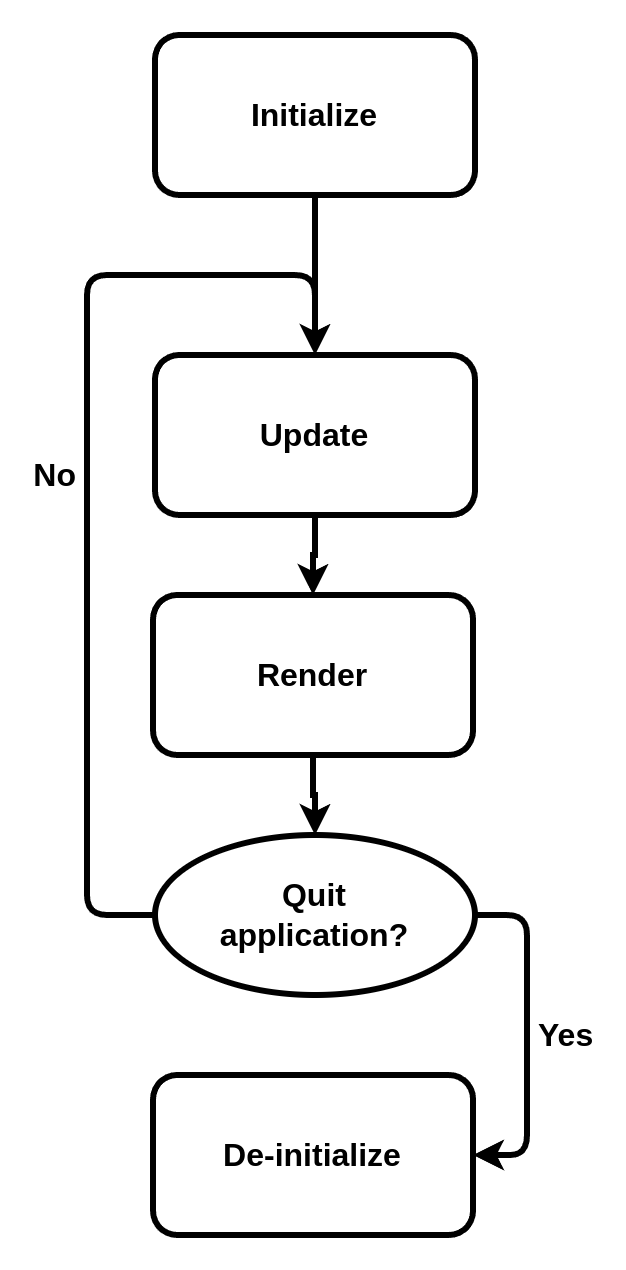
\includegraphics[scale=0.2]{resources/flow.png}
\end{figure}

Lo schema riporta le operazioni fondamentali necessarie per sviluppare un'applicazione grafica.

Una delle caratteristiche principali e più importanti della API è la semplicità. È importante che l'utente che farà uso di XrBridge si possa concentrare il più possibile sullo sviluppare la propria applicazione invece di doversi occupare dei dettagli di implementazione della libreria. Questo significa che la API deve esporre solamente metodi e parametri che sono assolutamente necessari per l'utente e null'altro. Per questo motivo, è stato deciso di avere un solo metodo per ogni operazione fondamentale: inizializzazione, aggiornamento dello stato, render e de-inizializzazione. I dettagli della API e dei metodi si trovano nella documentazione apposita.

XrBridge è stato implementato sotto forma di una singola classe, dove ogni metodo pubblico rappresenta una delle operazioni fondamentali. Per facilitare l'utilizzo di XrBridge, oltre che ad offrire una documentazione più dettagliata della API e un'applicazione di essempio che ne dimostra chiaramente l'utilizzo, ogni metodo ha dei controlli per assicurarsi che essi vengono chiamati nell'ordine giusto (per esempio per assicurarsi che l'utente abbia inizializzato XrBridge prima di renderizzare una scena).

\subsection{Inizializzazione}

Il primo passo è quello di inizializzare XrBridge. Questo significa creare una connessione con la runtime di OpenXR, iniziare una sessione e caricare le estensioni necessarie. Il suddetto passo è assolutamente necessario per poter utilizzare le funzionalità di OpenXR. Un errore durante questa fase è probabilmente causato da un problema con l'ambiente di esecuzione; infatti potrebbe trattarsi di un errore di configurazione della runtime o di un problema con l'hardware VR. Nessun'altra azione può essere eseguita prima dell'inizializzazione e l'inizializzazione può avvenire una sola volta (inizializzare più volte è considerato un errore).

XrBridge mette a disposizione il metodo \texttt{bool init(std::string\& application\_name)} per fare questo. Il parametro \texttt{application\_name} non è di molta importanza e viene utilizzato da SteamVR solamente come dettaglio visivo e non ha alcun effetto sull'esecuzione dell'applicazione. Per i dettagli sul suo utilizzo, fare riferimento alla documentazione sulla API e all'applicazione di esempio.

\subsection{Update}

Questa è una delle operazioni che vengono eseguite per la duranta dell'applicazione. Il metodo \texttt{bool update()} si occupa principalmente di gestire gli eventi generati da OpenXR, come ad esempio la conclusione di una sessione.

È inoltre importante per l'utente costantemente monitorare il valore di ritorno di questa funzione, poichè un errore potrebbe essere sollevato nel caso la runtime si disconnetta (con ogni probabilità l'utente ha disconnesso il suo visore o ha chiuso la runtime prima di terminare l'applicazione).

OpenXR distingue tra un'istanza e una sessione. L'istanza è il collegamento alla runtime e viene creata una sola volta durante l'inizializzazione; mentre una sessione può essere terminata e ricreata più volte durante l'esecuzione dell'applicazione. Un'istanza viene generalmente distrutta quando la runtime stessa viene terminata; in questo caso, XrBridge segnala un errore e necessita di un riavvio dell'applicazione. Nel caso la sessione venisse invece terminata, XrBridge attenderà semplicemente che la sessione venga ristabilita senza segnalare alcun errore o output.

\subsection{Render}

Questo è il passo più complesso, rispettivamente è quello che differisce maggiormente rispetto a OvVR. Come update, anche render viene seguito di continuo. Il rendering consiste nel generare le immagini che verranno poi proiettate sul visore VR, seguendo le istruzioni dell'utente. L'utente invoca il metodo \texttt{render(render\_function\_t render\_function)} per renderizzare. L'argomento \texttt{render\_function} verrà spiegato più tardi.

OpenXR ha un sistema di rendering molto complesso che prende in considerazione la tempistica dei frame (refresh-rate), layers e swapchains.

OpenXR si aspetta che alcune azioni vengano eseguite entro un tempo limite stabilito dalla runtime. Nel caso il tempo limite scada, le conseguenze dipendono anche loro dalla runtime. Questo si applica anche al rendering dei frame. Nel caso di SteamVR, un mancato tempo limite potrebbe risultare in difetti grafici. Questa sincronizzazione è fatta dalla funzione \texttt{xrWaitFrame}.

Per costruire un frame, OpenXR utilizza un sistema di layers. Esistono diversi tipi di layers (3D, 2D, ...) che verranno poi sovrapposti (composizione) dalla runtime per generare l'immagine finale. È per esempio possibile avere un layer 2D dedicato alla GUI e un altro layer 3D per la scena. È anche posibilie utilizzare un singolo layer 3D e disegnare la GUI manualmente senza affidarsi alla composizione offerta da OpenXR. Questo è l'approccio di XrBridge, dove viene utilizzato un singolo layer di proiezione (layer 3D).

Il layer di proiezione si aspetta un certo numero di \textit{view}. Una view consiste in un'immagine che verrà mostrata sul dispositivo VR. Nel caso di un headset, ci saranno due view: una per l'occhio destro e l'altra per l'occhio sinistro. È dunque necessario renderizzare la scena per ciascun occhio.

Quando si tratta di rendering, una delle maggiori differenze tra OpenVR e OpenXR, è chi si occupa di generare i framebuffer che verranno utilizzati per il rendering. Nel caso  di OpenVR, è compito dell'utente creare i framebuffers, riempirli e inviarli a OpenVR una volta che il rendering è completo. Al contraro, OpenXR esige che sia la runtime a creare i framebuffers e che l'utente deve richiedere i framebuffers prima di poterli utilizzare. Questa differenza cambia in modo significativo la struttura dell'applicazione dal punto di vista del corso di realtà virtuale. Se prima gli studenti dovevano imparare a creare i propri framebuffer, ora questo processo è automatico.

Di seguito è riportata la sequenza di azioni richieste da OpenXR per renderizzare una scena. Le parti in italico sono implementate dall'utente, mentre il resto è eseguito automaticamente da XrBridge.

\begin{enumerate}
  \item Attendere il momento giusto per iniziare a renderizzare il frame (sincronizzazione).
  \item Preparare il rendering dell'intero frame (begin).
  \item Preparare il rendering dell'occhio \textbf{sinistro} (begin).
  \item \textit{Renderizzare la scena dalla propsettiva dell'occhio sinistro}.
  \item Finalizzare il rendering dell'occhio sinistro (end).
  \item Preparare il rendering dell'occhio \textbf{destro} (begin).
  \item \textit{Renderizzare la scena dalla propsettiva dell'occhio destro}.
  \item Finalizzare il rendering dell'occhio destro (end).
  \item Finalizzare il rendering dell'intero frame (end).
\end{enumerate}

Il frame è mostrato all'utente solamente alla fine di tutta la procedura di render, quando tutte le view sono complete.

Come si può notare, ci sono due sequenze di \textit{begin - ... - end}: una per l'intero frame e una per ogni view/occhio.

Una possibilità di implementazione consiste nell'avere un metodo per ogni fase, come ad esempio \textit{begin\_frame}, \textit{begin\_eye}, \textit{end\_eye}, \textit{end\_frame}. Questa soluzione pone alcuni problemi:

\begin{itemize}
  \item Una grande quantità di metodi sono richiesti;
  \item Questo richiede che l'utente faccia molta attenzione che ogni metodo venga chiamato nell'ordine corretto, il che aumenta la complessità e il rischio di sbagli;
  \item Questo approccio non è scalabile (cosa succederebbe se si volesse adattare XrBridge per sviluppare un'applicazione con una sola view?);
  \item È complesso da implementare ed è poco elegante.
\end{itemize}

Per XrBridge è stato scelto un approccio che appare molto più pulito, ordinato, semplice e scalabile: l'utente fornisce una propria funzione di render che verrà invocata quante volte necessario da XrBridge. È possibile utilizzare una lambda per questo, come nell'esempio seguente (semplificato):

\begin{verbatim}
  void render()
  {
    // ...
    xrbridge.render([&] (
      Eye eye,
      shared_ptr<Fbo> fbo,
      mat4 proj_matrix,
      mat4 view_matrix,
      uint32_t width,
      uint32_t height)) {

      // Render scene

    });
    // ...
  }
\end{verbatim}

Per più dettagli sul metodo e gli argomenti, fare riferimento alla documentazione di XrBridge.

Lo svantaggio principale riguardo questo approccio è il fatto che richiede una minima conoscenza delle lambda.

Per contro, un grande vantaggio (che si può notare dall'esempio), è il fatto che, ogni volta che la lambda viene chiamata, è semplice reperire tutte le informazioni necessarie per renderizzare la scena: questo include il framebuffer da utilizzare, le matrici di proiezione e view e altri parametri che si possono aggiungere se desiderato, senza necessitare di grandi modifiche al codice. Questo permette maggiormente di semplificare la API, dal momento che non sono necessari metodi appositi per recuperare le informazioni. Ad ogni chiamata della lambda, tutte le informazioni necessarie sono subito a disposizione. Utilizzando la lista di cattura della lambda (e catturando tutto il contesto come mostrato nell'esempio sopra), ciò permette di eseguire operazioni di preparazione una sola volta (ad esempio costruire la lista di render) invece di sprecare risorse e ripetere le stesse operazioni per ogni chiamata della lambda. Se utilizzato in questo modo, dal punto di vista dell'utente, questo approccio diventa molto semplice da comprendere e implementare, rispettivamente permette di ignorare quasi completamente le complessità che nascono dall'utilizzo di lambda.

Lo svantaggio di passare le matrici in questo modo, però, è il fatto che le matrici vengono ottenute solamente al momento del rendering e non possono essere ottenute indipendentemente. Di conseguenza, una possibile logica che faccia uso delle matrici (ad esempio per verificare la posizione dell'utente), dovrà essere eseguita al momento del rendering.

\subsection{De-inizializzazione}

Si tratta dell'ultimo passaggio, dopo il quale l'istanza di XrBridge diventerà inutilizzabile. A questo punto l'utente dovrà riavviare l'applicazione oppure creare una nuova istanza. Il metodo \texttt{bool free()} si occupa di terminare la sessione, l'istanza e liberare tutte le risorse utilizzate.

\subsection{Gestione errori}

Esistono svariati approcci alla gestione degli errori nel codice. I due approcci più comuni sono \textit{exceptions} e \textit{errors as values}. Per questo progetto è stato scelto il secondo approccio, per alcuni motivi: 1) è lo stesso approccio utilizzato da OvVR; 2) è lo stesso approccio utilizzato da OpenXR; 3) è più semplice rispetto alle eccezioni; 4) non vi è nessuna interruzione inaspettata del flusso di esecuzione.

Tutti i metodi di XrBridge seguono quindi la stessa convenzione: ritornano un valore \texttt{true} se il metodo è stato eseguito con successo e \texttt{false} in caso di errore. Inoltre, in caso di un errore, un messaggio che descrive l'errore viene stampato su \textit{stderr}.

\section{OpenXR}

\subsection{Layers e estensioni}

Similmente a Vulkan, OpenXR permette di estendere le proprie funzionalità attraverso dei layers e delle estensioni.

Un layer, come suggerisce il nome, è uno strato che può essere inserito fra OpenXR e l'applicazione. Un layer può offrire funzionalità come ad esempio il tracciamento delle chiamate delle funzioni. Per questo progetto, non è stato necessario nessun layer. In caso si voglia aggiungere un layer, è sufficiente aggiungere il suo nome alla riga seguente all'interno di \texttt{xrbridge.cpp}, nella funzione \texttt{init}:

\begin{verbatim}
  const std::vector<std::string> requested_api_layers = { };
\end{verbatim}

Le estensioni, invece, permettono di aggiungere funzionalità extra a OpenXR. Alcune estensioni sono sviluppate da Khronos, ma possono anche essere sviluppate da terze parti. Per questo progetto, una singola estensione è stata necessaria: \texttt{XR\_KHR\_opengl\_enable}. Come suggerisce il nome, questa estensione abilita il supporto per la API grafica OpenGL.In caso si voglia aggiungere un'altra estensione, è sufficiente aggiungere il suo nome alla riga seguente all'interno di \texttt{xrbridge.cpp}, nella funzione \texttt{init}:

\begin{verbatim}
  const std::vector<std::string> requested_extensions = {
    "XR_KHR_opengl_enable",
  };
\end{verbatim}

\subsection{Binding grafico}

OpenXR fa uso di "graphic bindings", ovvero strutture che legano insieme una API grafica e una piattaforma. All'interno del codice, questi binding sono implementati sotto forma di struct. Esiste uno struct per ogni combinazione di API grafica (OpenGL, Vulkan, DirectX, ...) e piattaforma (Win32, X11, Wayland, ...) supportate. Ogni struct richiede dei parametri legati alla piattaforma e alla API grafica scelta. Questi struct sono definiti nel file \texttt{openxr\_platform.h} della libreria OpenXR. Ecco alcuni esempi:

\begin{table}[H]
  \caption{Strutture per il binding grafico}
  \begin{center}
    \begin{tabular}{ l l l }
      API grafica & Piattaforma & Nome struct \\
      \hline
      OpenGL      & Windows         & \texttt{XrGraphicsBindingOpenGLWin32KHR} \\
      OpenGL      & Linux (Xlib)    & \texttt{XrGraphicsBindingOpenGLXlibKHR} \\
      OpenGL      & Linux (Wayland) & \texttt{XrGraphicsBindingOpenGLWaylandKHR}
    \end{tabular}
  \end{center}
\end{table}

Durante l'inizializzazione di OpenXR, è compito dello sviluppatore istanziare e configurare uno di questi stuct per la piattaforma che si vuole utilizzare. I requisiti richiedono solo il supporto per OpenGL su Windows e Linux. Di seguito sono descritti gli approcci all'implementazione dei binding richiesti.

\subsubsection{Binding OpenGL + Windows}

Di seguito è riportata la definizione della struttura che rappresenta il binding OpenGL + Windows (i parametri \texttt{type} e \texttt{next} non sono importanti per questo capitolo):

\begin{verbatim}
  typedef struct XrGraphicsBindingOpenGLWin32KHR {
    XrStructureType             type;
    const void* XR_MAY_ALIAS    next;
    HDC                         hDC;
    HGLRC                       hGLRC;
  } XrGraphicsBindingOpenGLWin32KHR;
\end{verbatim}

I due parametri più importanti sono \texttt{hDC} e \texttt{hGLRC} e fanno parte della API Win32. \texttt{hDC} indica il \textit{device context}, mentre \texttt{hGLRC} è il \textit{OpenGL Rendering Context}; non è importante cosa rappresentano questi parametri, ma è necessario averli.

Qui si incontra però un ostacolo: il contesto di OpenGL viene generato automaticamente da FreeGLUT. Per questioni di portabilità, FreeGLUT non offre un modo di recuperare questi parametri; in questo contesto servono gli stessi parametri che FreeGLUT \footnote{FreeGLUT è una libreria che si occupa di gestire finestre grafiche, input e contesti OpenGL.} ha usato per creare il contesto OpenGL, il che significa che non possiamo generare un nuovo contesto, rispettivamente generare nuovi parametri. Fortunatamente, la API Win32 di Windows offre un metodo per recuperare entrambi i parametri, questo grazie alle funzioni \texttt{wglGetCurrentDC} e \texttt{wglGetCurrentContext}. Grazie a queste funzioni, è possibile configurare tutta la struct e, di conseguenza, configurare OpenXR per questa piattaforma.

\subsubsection{Binding OpenGL + Linux}

Questo binding è più complesso e complicato rispetto a quello di OpenGL + Windows per due motivi.

a) Linux non ha una API standard per quanto riguarda gli ambienti grafici. b) Al momento esistono due principali piattaforme grafiche su Linux: X11 e Wayland. Inoltre, per X11, esistono approcci diversi per ognuna delle due librerie X11 più diffuse: Xcb e libX.

Per questo motivo, esistono tre struct per il binding OpenGL + Linux:

\begin{itemize}
  \item \texttt{XrGraphicsBindingOpenGLXlibKHR} (LibX)
  \item \texttt{XrGraphicsBindingOpenGLXcbKHR} (Xcb)
  \item \texttt{XrGraphicsBindingOpenGLWaylandKHR} (Wayland)
\end{itemize}

Inizialmente era stato deciso di utilizzare Wayland per due motivi. Il primo motivo è che lo struct per questo binding richiede un solo parametro, apparentemente rendendo più semplice l'implementazione. Il secondo motivo è il fatto che Wayland sta andando sempre di più a sostituire X11, tanto che molte delle distribuzioni di Linux principali supportano Wayland out-of-the-box. Lo svantaggio però è il fatto che non è possibile eseguire applicazioni Wayland su X11. Questo approccio non è stato pertanto possibile a causa dell'assenza di supporto per Wayland in FreeGLUT. Nonostante FreeGLUT abbia un'implementazione di Wayland, come anche suggerito da un commento di uno degli sviluppatori \footnote{\url{https://github.com/freeglut/freeglut/issues/164\#issuecomment-2091892089}}, tale implementazione non è funzionante e sembra al momento abbandonata. A causa dei problemi appena menzionati, ho deciso di utilizzare l'approccio con X11.

Fortunatamente, esiste un software dal nome di XWayland che permette di eseguire quasi perfettamente molte applicazioni sviluppate per X11 in un ambiente Wayland. Usando l'approccio X11, quindi, sarà possibile supportare entrambe le piattaforme X11 e Wayland.

Per quanto riguarda l'approccio X11, esistono due alternative: a) utilizzare la libreria Xlib \footnote{Libreria originale per interagire con X11} b) Xcb \footnote{Libreria alternativa a Xlib}. Tra i due approcci, utilizzare Xlib è il più semplice e diretto, poichè non richiede di stabilire una connessione a X11. Di seguito è riportato lo struct per il binding OpenGL + Linux (X11):

\begin{verbatim}
  typedef struct XrGraphicsBindingOpenGLXlibKHR {
      XrStructureType             type;
      const void* XR_MAY_ALIAS    next;
      Display*                    xDisplay;
      uint32_t                    visualid;
      GLXFBConfig                 glxFBConfig;
      GLXDrawable                 glxDrawable;
      GLXContext                  glxContext;
  } XrGraphicsBindingOpenGLXlibKHR;
\end{verbatim}

I parametri \texttt{xDisplay}, \texttt{glxDrawable} e \texttt{glxContext} sono facilmente reperibili utilizzando le funzioni \texttt{glXGetCurrentDisplay}, \texttt{glXGetCurrentDrawable} e \texttt{glXGetCurrentContext} rispettivamente. Il problema sono i parametri \texttt{visualid} e \texttt{glxFBConfig}. Anche questi sono parametri che sono configurati da FreeGLUT ma non sono esposti e non esiste un modo per recuperarli come è possibile per i parametri precedenti.

\subsection{Istanze e sessioni}

OpenXR fa distinzione fra un'istanza e una sessione. Mentre un'istanza è semplicemente una connessione a OpenXR che viene creata una volta all'avvio dell'applicazione e terminata alla fine, una sessione è più complessa. Una sessione può essere terminata e ripresa in qualsiasi momento, ma esiste una sola sessione per istanza e, rispettivamente, una sola istanza per istanza di XrBridge. L'istanza di OpenXR è creata nel metodo \texttt{bool init()} e distrutta nel metodo \texttt{bool free()}.

Alcuni elementi, come ad esempio lo spazio di riferimento e le swapchain (vedi sezione successiva), sono legati alla sessione e perciò verranno creati e distrutti insieme alla sessione.

L'inizio e la fine di una sessione è deciso interamente dalla runtime ed è comunicato all'applicazione attraverso degli eventi. Il metodo \texttt{bool update()} si occupa proprio di rispondere ai vari eventi generati da OpenXR, incluso l'inizio e la fine della sessione.

Appena viene ricevuto un evento di inizio o fine sessione, viene chiamato il metodo \texttt{bool begin\_session()} o \texttt{bool end\_session()} rispettivamente.

\subsection{Swapchain}

Una swapchain in OpenXR è una serie di una o più immagini utilizzate per il rendering, dove il numero di immagini in una swapchain dipende dalla configurazione della runtime. Per esempio, se la runtime è configurata per utilizzare la tecnica \textit{double buffering}, una swapchain sarà composta di due immagini, mentre se la runtime utilizza il \textit{triple buffering}, le swapchain avranno tre immagini.

Il formato delle immagini è definito dall'utente e dipende dalla API grafica utilizzata, mentre le immagini vere e proprie vengono create dalla runtime (questo è il comportamento opposto rispetto a OpenVR, dove è l'utente che si deve occupare di creare le immagini, renderizzarle e inviarle alla runtime). Durante la creazione di una swapchain l'utente può scegliere altri parametri, come ad esempio la dimensione delle immagini. Lo standard di OpenXR non specifica quali formati di immagini le runtime devono supportare e, perciò, l'utente deve scegliere un formato che è supportato dalla runtime che desidera utilizzare. In una swapchain, le immagini sono salvate in ordine e ogni immagine ha un indice che la distingue dalle altre immagini della stessa swapchain.

Un'applicazione VR può avere una o più "view", dove una view consiste in una "schermata". Nel caso di un'applicazione che fa uso di un visore del tipo "head-mounted", esisteranno due view: una per ciascun occhio. Nel caso di un sistema cave, esisterà una view per ogni lato. Ogni view ha una swapchain e, di conseguenza, il numero totale di immagini sarà $ {N}_{immagini} = {N}_{view} \times k $, dove $ k $ è il numero di immagini per view (esempio: 2 nel caso di double-buffering). Per questo progetto, è richiesto che solamente due view siano supportate.

Quando è il momento di renderizzare, l'utente deve richiedere alla runtime quale immagine di una swapchain deve utilizzare; la runtime risponderà con un indice. Se, per esempio, una swapchain ha tre immagini, la runtime ritornerà all'utente un indice 0, 1 o 2. L'utente deve quindi utilizzare quella immagine per renderizzare. Una volta terminato, l'utente "rilascia" l'immagine alla runtime che si occuperà poi di mostrare l'immagine sul visore VR. Al prossimo ciclo di rendering, la runtime fornirà un'altra immagine all'utente da utilizzare. Dalle mie osservazioni di SteamVR, l'ordine delle imagini fornite è: 0, 1, 2, 0, 1, 2, 0, 1, 2, ...

\begin{figure}[H]
  \caption{Struttura di swapchain e view per un Head Mounted Display / 2 swapchain, 3 view per swapchain}
  \centering
  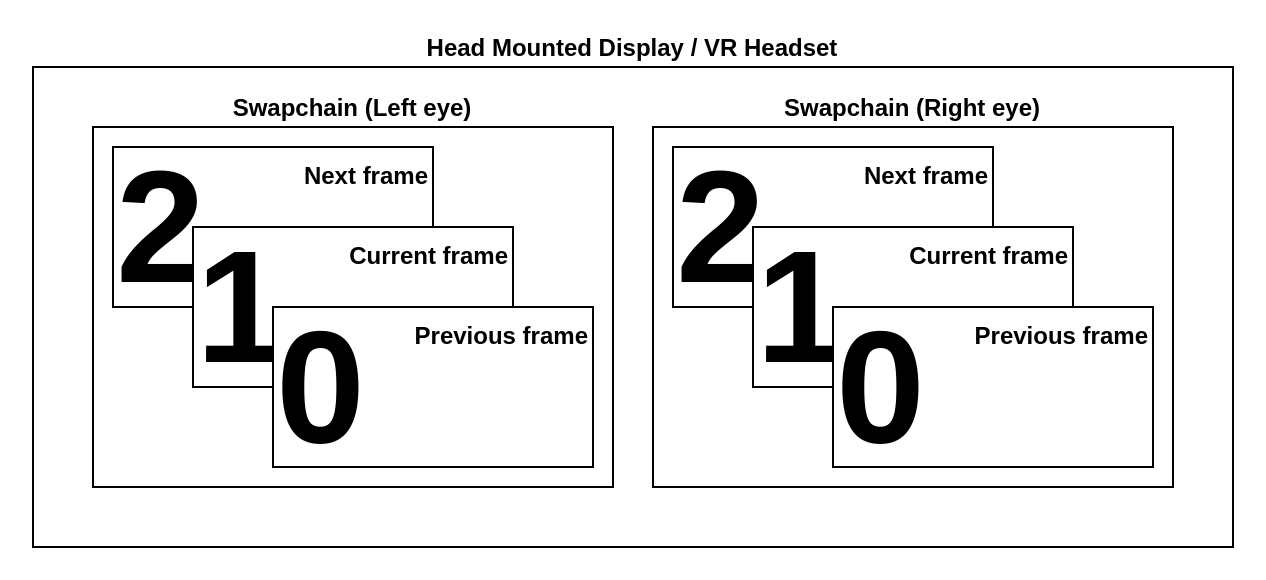
\includegraphics[scale=0.3]{resources/swapchains.png}
\end{figure}

Per praticità, all'interno del codice, è stata definita la struttura \texttt{Swapchain}, la quale aiuta a semplificare il codice legando insieme i vari componenti di una swapchain: la lista delle immagini, la dimensione delle immagini e la struttura \texttt{XrSwapchain} di OpenXR.

Le swapchain vengono istanziate quando una sessione di OpenXR inizia, all'interno del metodo \texttt{bool begin\_session()}, una swapchain per view. Qui vengono create e configurate tutte le swapchain necessarie. Il metodo \texttt{shared\_ptr<Fbo> create\_fbo(GLuint w, GLuint h)} si occupa di generare le immagini (FBO = Frame Buffer Object) necessarie per le swapchain. Quest'ultimo fa affidamento alla classe \texttt{Fbo} già creata e utilizzata durante il corso di realtà virtuale dal docente responsabile. Questa classe consiste in un wrapper attorno agli FBO di OpenGL e ne semplifica l'utilizzo. Grazie a questo, gli utenti avranno meno difficoltà quando dovranno utilizzare i framebuffer durante il rendering.

Il numero di swapchain è deciso in base alla \textit{view configuration type} \footnote{\url{https://registry.khronos.org/OpenXR/specs/1.0/man/html/XrViewConfigurationType.html}}. I due tipi di configurazione principali sono \textit{mono} e \textit{stereo}. Mono significa una singola view; questo è il caso per un'applicazione di realtà aumentata, dove l'unica view è presa dalla telecamera del dispositivo e gli oggetti virtuali vengono sovrapposti al mondo reale. Stereo, invece, indica due view. Questo è il caso di un visore di realtà virtuale da indossare (effettivamente degli occhiali) e richiede due view: una per l'occhio sinistro e una per l'occhio destro. XrBridge supporta solamente la configurazione stereo; è possibile però modificare il tipo di configurazione apportando poche e piccole modifiche. Questa configurazione è fatta all'inizio del metodo \texttt{bool begin\_session()}.

I framebuffer generati sono composti da una texture generata da OpenXR e il cui formato è specificato dall'utente e un buffer di profondità.

\subsection{Spazio di riferimento}

In OpenXR, lo spazio di riferimento (\texttt{XrReferenceSpaceType} \footnote{\url{https://registry.khronos.org/OpenXR/specs/1.1/man/html/XrReferenceSpaceType.html}}) è il sistema con cui un'applicazione VR tiene traccia della posizione e rotazione del mondo reale.

Nel codice, lo spazio di riferimento è configurato durante la creazione di una sessione, alla fine del metodo \texttt{bool begin\_session()} dopo la creazione delle swapchain. Lo spazio di riferimento utilizzato può essere configurato attraverso la variabile \texttt{XRBRIDGE\_CONFIG\_SPACE} nella sezione di configurazione iniziale in \texttt{xrbridge.cpp}.

Di seguito sono riportati i principali spazi di riferimento disponibili in OpenXR senza fare uso di estensioni:

\begin{table}[H]
  \caption{Tipi di spazi di riferimento}
  \begin{center}
    \begin{tabular}{ m{7cm} m{6cm} }
      Nome                                             & Descrizione \\
      \hline
      \texttt{XR\_REFERENCE\_SPACE\_TYPE\_VIEW}        & Questo spazio non tiene conto della rotazione e posizione dell'utente. Utile per implementare una GUI. \\
      \texttt{XR\_REFERENCE\_SPACE\_TYPE\_LOCAL}       & Questo spazio posiziona l'utente all'origine della scena. \\
      \texttt{XR\_REFERENCE\_SPACE\_TYPE\_STAGE}       & \textbf{Default}. Questo spazio posiziona l'utente relativo all'origine dello spazio reale configurato all'interno della runtime. \\
    \end{tabular}
  \end{center}
\end{table}

\begin{figure}[H]
  \begin{minipage}{.3\textwidth}
    \centering
    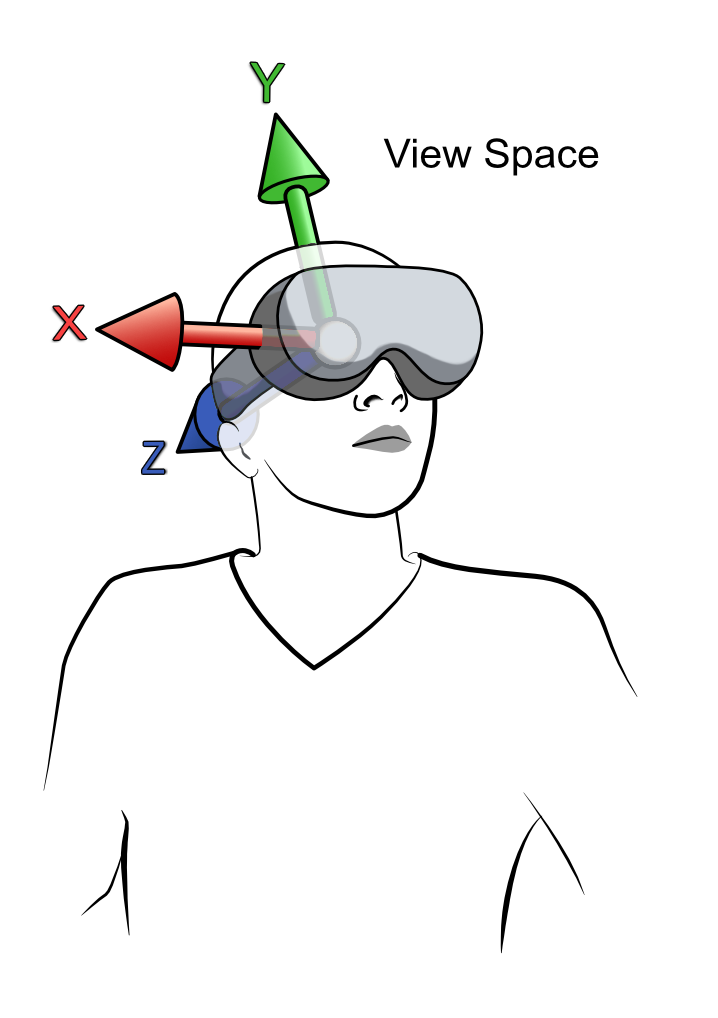
\includegraphics[width=.9\linewidth]{resources/view_space.png}
    \caption{Spazio di riferimento VIEW}
  \end{minipage}
  \begin{minipage}{.3\textwidth}
    \centering
    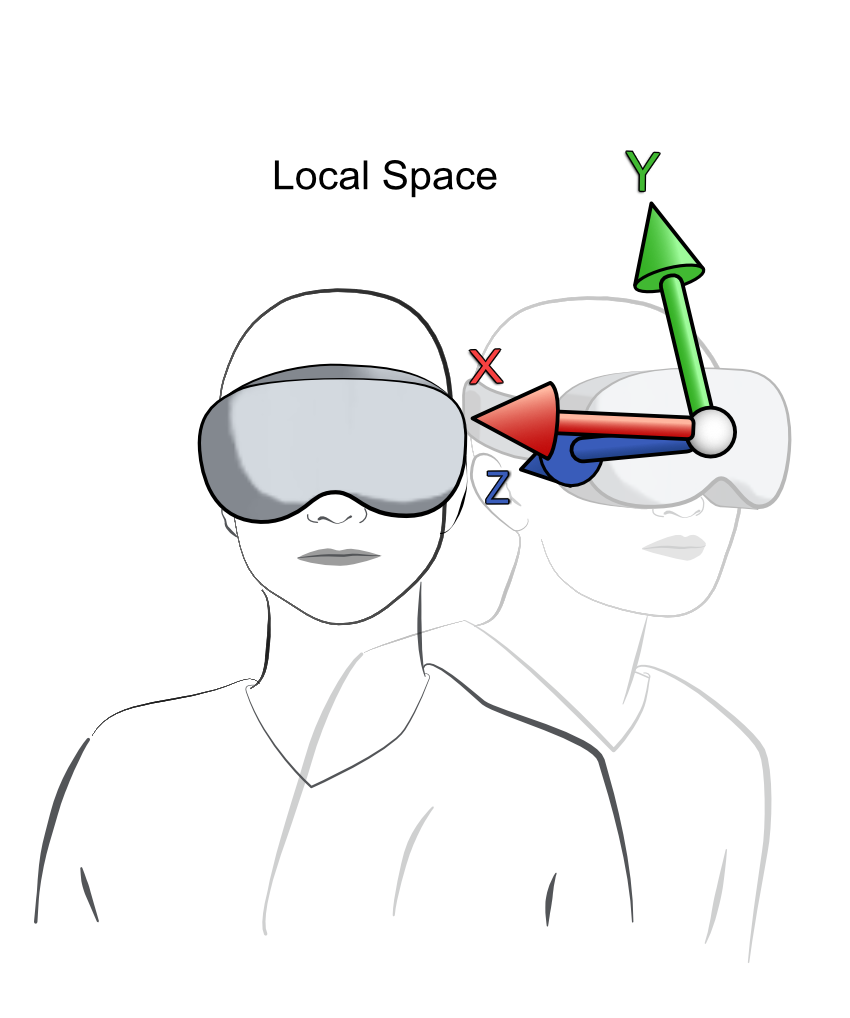
\includegraphics[width=.9\linewidth]{resources/local_space.png}
    \caption{Spazio di riferimento LOCAL}
  \end{minipage}
  \begin{minipage}{.3\textwidth}
    \centering
    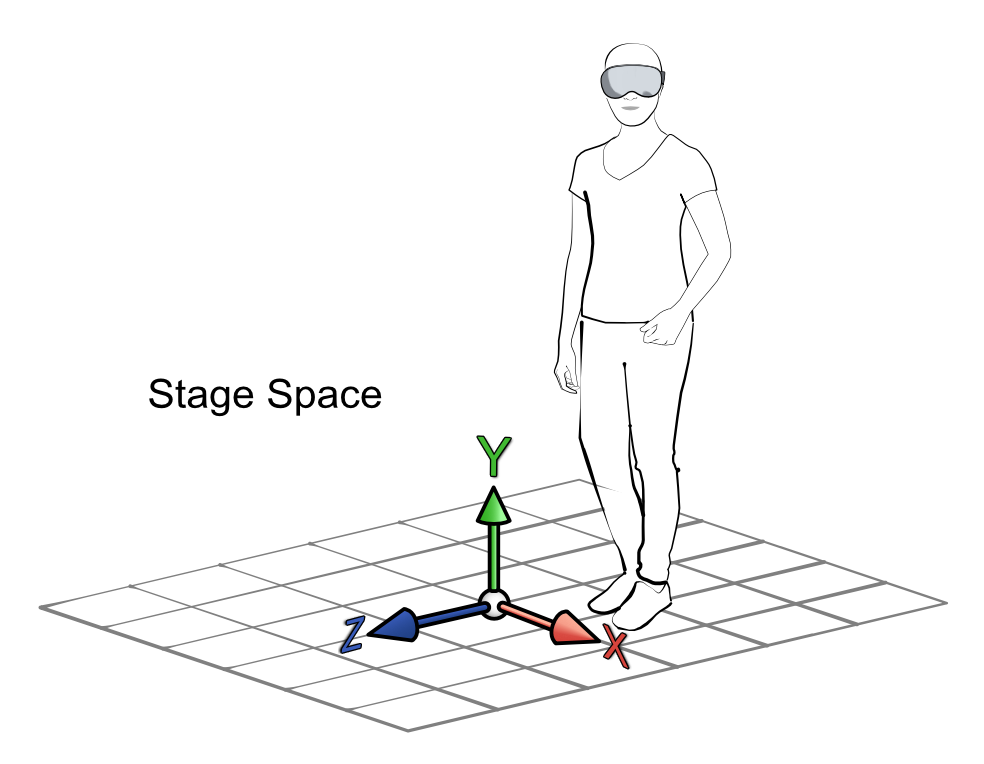
\includegraphics[width=.9\linewidth]{resources/stage_space.png}
    \caption{Spazio di riferimento STAGE}
  \end{minipage}
\end{figure}

Le immagini sono state prese dal tutorial ufficiale \footnote{\url{https://openxr-tutorial.com/linux/opengl/3-graphics.html\#reference-spaces}}.

\subsection{Matrice di view}

OpenXR non genera automaticamente le matrici di view e prospettiva necessarie per renderizzare, bensì, fornisce una serie di parametri che possono essere utilizzati per successivamente costruire le matrici necessarie.

Al momento del rendering, OpenXR offre un'istanza della struttura \texttt{XrView} \footnote{\url{https://registry.khronos.org/OpenXR/specs/1.0/man/html/XrView.html}} contenente la posizione, rotazione e FOV (Field Of View) della view attuale (in altre parole, le coordinate dell'occhio nella scena). La posizione è espressa da un vettore (unità in metri), mentre la rotazione è espressa da un quaternione unitario. La posizione e la rotazione sono contenute nella struttura \texttt{XrPosef} \footnote{\url{https://registry.khronos.org/OpenXR/specs/1.0/man/html/XrPosef.html}}. Di seguito è mostrata la procedura utilizzata per convertire posizione e rotazione in una singola matrice di view. La macro \texttt{XRV\_TO\_GV} serve a convertire un vettore \texttt{XrVector3f} di OpenXR in un vettore \texttt{glm::vec3} di GLM. Inoltre, l'ordine delle operazioni è dettato dalla specifica. La libreria GLM permette di semplificare la creazione e le operazioni sulle matrici. Quanto sopra viene ripetuto per ogni occhio (sinistro e destro).

\begin{verbatim}
  glm::mat4 rotation_matrix = glm::mat4_cast(quaternion);
  glm::mat4 translation_matrix = glm::translate(glm::mat4(1.0f),
    XRV_TO_GV(current_view.pose.position));
  glm::mat4 view_matrix = translation_matrix * rotation_matrix;
\end{verbatim}

\subsection{Matrice di proiezione}

La matrice di proiezione, invece, è più complessa rispetto alla matrice di view e, in più, non è possibile affidarsi a GLM.

Nonostante GLM metta a disposizione la funzione \texttt{glm::perspective}, la quale permette di generare una matrice di prospettiva simmetrica, OpenXR richiede una matrice di proiezione non simmetrica.

Per ovviare a questo problema è stato creato il metodo \texttt{create\_projection\_matrix}. Attraverso la struttura \texttt{XrFovf} \footnote{\url{https://registry.khronos.org/OpenXR/specs/1.0/man/html/XrFovf.html}} è possibile reperire gli angoli necessari per costruire la matrice di proiezione. Infine, utilizzando il metodo apposito \texttt{create\_projection\_matrix} definito in \texttt{xrbridge.cpp}, si costruisce la matrice di proiezione finale.

\begin{verbatim}
  glm::mat4 projection_matrix = create_projection_matrix(
    current_view.fov,
    this->near_clipping_plane,
    this->far_clipping_plane);
\end{verbatim}

Per ultimo, la matrice di view e quella di proiezione vengono passate alla funzione di render fornita dall'utente, assieme a tutti gli altri parametri:

\begin{verbatim}
  render_function(
    eye,
    fbo,
    projection_matrix,
    view_matrix,
    current_swapchain.width,
    current_swapchain.height);
\end{verbatim}

Questo permette di renderizzare la scena dal punto di vista di ciascun occhio.

\section{Limitazioni di FreeGLUT}

FreeGLUT è una libreria multi-piattaforma che permette di gestire finestre, contesti OpenGL, mouse e tastiera. L'utilizzo di questa libreria è obbligatoria dal momento che viene utilizzata durante i corsi di grafica e di realtà virtuale. Per questo progetto, è stata utilizzata la versione 3.6.0.

L'utilizzo di FreeGLUT è obbligatorio dal momento che fa già parte del corso di grafica. In più, FreeGLUT offre alcune funzionalità extra che facilitano lo sviluppo di applicazioni grafiche nel corso, come ad esempio l'abilità di scrivere del testo direttamente sullo schermo oppure la presenza di primitive geometriche immediatamente utilizzabili senza necessitare di programmi di modellazione 3D.

Come menzionato in precedenza nel capitolo \textit{Binding OpenGL + Linux}, FreeGLUT non espone certi parametri che potrebbero essere necessari ad un'applicazione. È stato dunque necessario apportare modifiche alla libreria. Di seguito è descritto l'approccio scelto.

È stato aggiunto un nuovo file a FreeGLUT chiamato \texttt{/include/GL/freeglut\_globals.h} e, al suo interno, sono state definite due variabili globali:

\begin{verbatim}
  // Etratto da freeglut_globals.h
  #pragma once

  static uint32_t freeglut_visualid = 0;
  static int freeglut_attributes[100] = { 0 };
\end{verbatim}

All'interno di XrBridge, è stato successivamente incluso questo file header per accedere alle variabili globali. Come parte della consegna del progetto, è anche presente una patch di git che descrive i cambiamenti effettuati nel dettaglio, così da poter essere facilmente applicati e analizzati. È importante prestare attenzione al fatto che la patch non contiene la creazione del nuovo file.

\begin{quote}
  Attenzione al fatto che la versione modificata di FreeGLUT è stata verificata solamente su Linux; per utilizzare FreeGLUT su Windows, utilizzare la versione originale non modificata.
\end{quote}

Iniziando con il parametro più semplice: \texttt{visualid}. Si tratta di un semplice valore \texttt{uint32\_t}.

È bastato aggiungere una singola riga di codice che assegna alla variabile globale creata il valore della variabile \texttt{visualInfo->visualid}. Questo viene fatto all'interno della funzione \texttt{fgPlatformOpenWindow} nel file \texttt{src/x11/fg\_window\_x11.c}.

\begin{verbatim}
  // src/x11/fg_window_x11.c @ 432
  freeglut_visualid = visualInfo->visualid;
\end{verbatim}

Il secondo parametro è \texttt{glxFBConfig}. Questo è più complicato rispetto al precedente, perché non si tratta di un semplice valore che può essere facilmente copiato, bensì di una struttura interna che non viene esposta all'utente se non attraverso un puntatore. Questa struttura viene generata dalla funzione \texttt{glXChooseFBConfig}, la quale accetta una serie di attributi assieme ad altri parametri e ritorna un puntatore ad una struttura di tipo \texttt{GLXFBConfig}. La soluzione è fortunatamente piuttosto semplice: è sufficiente ottenere la lista di attributi usati per generare la struttura e invocare nuovamente il metodo \texttt{GLXFBConfig}. Per fare questo, è stato necessario salvare gli attributi in una delle variabili globali appena create. Questo è stato fatto nella funzione \texttt{fghChooseConfig} nel file \texttt{src/x11/fg\_window\_x11\_glx.c}. Infine, all'interno di XrBridge, è bastato chiamare la funzione \texttt{glXChooseFBConfig} con gli attributi corretti. Così facendo si ottiene la struttura necessaria.

\begin{verbatim}
  // src/x11/fg_window_x11_glx.c @ 102
  for (unsigned int i = 0; i < 100; ++i)
  {
    freeglut_attributes[i] = attributes[i];
  }
\end{verbatim}

Una libreria alternativa a FreeGLUT è GLFW, la quale espone i parametri interni attraverso dei metodi specifici. Come menzionato all'inizio del capitolo, però, non è stato possibile utilizzare questa libreria.

\section{Differenze fra piattaforme Windows e Linux}

Ci sono alcune importanti differenze fra le piattafrome Windows e Linux che hanno richiesto aggiustamenti all'interno del codice. In precedenza è già stato menzionato come il binding grafico differisce tra piattaforme; di seguito saranno presentate alcune differenze che hanno causato difficoltà nello sviluppo di XrBridge.

Quando si tratta di generare i framebuffers per ogni view/occhio, è possibile specificare il formato dell'immagine desiderato (es: GL\_RGBA16F, GL\_SRGB8, ...). Il formato dipende fortemente dalla API grafica scelta e la runtime, dal momento che OpenXR non specifica alcun formato di default.

\newpage

Una delle difficoltà riscontrate durante lo sviluppo, è il fatto che SteamVR supporta formati diversi a seconda della piattaforma. Di seguito sono elencati alcuni dei formati supportati dalla versione attuale di SteamVR (2.7.4 su Windows e Linux; non sono state verificate le versioni beta):

\begin{table}[H]
  \caption{Formati immagine di OpenGL supportati da SteamVR}
  \begin{center}
    \begin{tabular}{ l l l }
      Formato                    & Windows & Linux \\
      \hline
      \texttt{GL\_RGB8}          & No      & No    \\
      \texttt{GL\_RGB16}         & No      & No    \\
      \texttt{GL\_RGBA8}         & No      & No    \\
      \texttt{GL\_RGBA16}        & Sì      & No    \\
      \texttt{GL\_RGB8\_SNORM}   & No      & No    \\
      \texttt{GL\_RGB16\_SNORM}  & No      & No    \\
      \texttt{GL\_RGBA8\_SNORM}  & No      & No    \\
      \texttt{GL\_RGBA16\_SNORM} & No      & No    \\
      \texttt{GL\_RGB16F}        & Sì      & No    \\
      \texttt{GL\_RGB32F}        & No      & No    \\
      \texttt{GL\_RGBA16F}       & Sì      & No    \\
      \texttt{GL\_RGBA32F}       & No      & No    \\
      \texttt{GL\_RGB8I}         & No      & No    \\
      \texttt{GL\_RGB16I}        & No      & No    \\
      \texttt{GL\_RGB32I}        & No      & No    \\
      \texttt{GL\_RGB8UI}        & No      & No    \\
      \texttt{GL\_RGB16UI}       & No      & No    \\
      \texttt{GL\_RGB32UI}       & No      & No    \\
      \texttt{GL\_RGBA8I}        & No      & No    \\
      \texttt{GL\_RGBA16I}       & No      & No    \\
      \texttt{GL\_RGBA32I}       & No      & No    \\
      \texttt{GL\_RGBA8UI}       & No      & No    \\
      \texttt{GL\_RGBA16UI}      & No      & No    \\
      \texttt{GL\_RGBA32UI}      & No      & No    \\
      \texttt{GL\_SRGB8}         & Sì      & Sì    \\
      \texttt{GL\_SRGB8\_ALPHA8} & Sì      & Sì    \\
      \texttt{GL\_RGB9\_E5}      & No      & No    \\
    \end{tabular}
  \end{center}
\end{table}

SteamVR è costantemente aggiornato e, perciò, è molto probabile che in futuro i formati supportati cambino.

Se si dovesse scegliere un formato non valido, verrà generato il seguente errore all'inizio di una sessione:  \texttt{XR\_ERROR\_SWAPCHAIN\_FORMAT\_UNSUPPORTED} (-26).

A causa di queste differenze, è stato deciso di permettere all'utente di specificare il formato per piattaforma invece di avere una singola configurazione globale.

Nella sezione di configurazione di XrBridge (all'inizio del file \texttt{xrbridge.cpp}) è possibile specificare il formato con le variabili \texttt{XRBRIDGE\_CONFIG\_SWAPCHAIN\_FORMAT\_WINDOWS} e \texttt{XRBRIDGE\_CONFIG\_SWAPCHAIN\_FORMAT\_LINUX}.

\section{Strumenti, librerie e versioni}

Di seguito sono riportate le versioni di tutti gli strumenti, software e librerie utilizzate per il progetto. Non sono necessariamente richieste le stesse identiche versioni per eseguire l'applicazione di demo o per utilizzare XrBridge.

\newpage

\begin{table}[H]
  \caption{Versioni di strumenti e librerie utilizzati}
  \begin{center}
    \begin{tabular}{ m{4cm} m{2cm} m{7cm} }
      Strumento & Versione & Note \\
      \hline
      ALVR & 20.8.0 & Software per Windows e Linux che permette di utilizzare un dispositivo Android come un headset. \\
      PhoneVR & 2.0.0 & Software per Android che permette di utilizzare un dispositivo Android come un headset. \\
      SteamVR & 2.7.4 & Runtime di OpenXR sviluppata da Valve. \\
      Visual Studio Community 2022 & 17.11.1 & IDE per sviluppare su Windows. \\
      Code::Blocks & svn-r13524 & IDE per sviluppare su Linux. \\
      Windows 11 & 21H2 & Piattaforma di sviluppo Windows. \\
      Fedora 40 KDE & 6.10.6 & Piattaforma di sviluppo Linux. \\
      OpenXR & 1.0.0 & Versione di OpenXR utilizzata per sviluppare XrBridge. \\
      FreeGLUT & 3.6.0 & Libreria di supporto per OpenGL (utilizzata sia su Windows sia per la versione modificata per Linux). \\
      GLEW & 2.1.0 & Libreria di supporto per OpenGL (Windows). \\
      GLEW (glew) & 2.2.0 & Libreria di supporto per OpenGL (Linux). \\
      GLM & 1.0.1 & Libreria matematica per OpenGL (Windows).\\
      GLM (glm-devel) & 0.9.9 & Libreria matematica per OpenGL (Linux). \\
      OpenXR Loader & 1.1.37 & Loader per OpenXR (Windows, compilato manualmente). \\
      OpenXR Loader (openxr, openxr-devel) & 1.0.33 & Loader per OpenXR (Linux). \\
      Nvidia GTX 970 & & GPU utilizzata. \\
      Nvidia & 555.58.03 & Driver video per Nvidia. \\
      HTC Vive & & Visore VR. \\
      Samsung Galaxy Note 8 & Android 9 & Dispositivo Android usato come visore VR. \\
    \end{tabular}
  \end{center}
\end{table}

\chapter{Test e validazione}

A causa della natura puramente grafica del progetto, non è stato possibile implementare una procedura di test automatizzata. OpenXR è però una API molto pignola e, di conseguenza, segnala immediatamente ogni errore commesso. Uno sbaglio nell'utilizzo di OpenXR risulterebbe pertanto in un errore o una schermata nera.

Per sviluppare e verificare il corretto funzionamento di XrBridge, è stata sviluppata una piccola, semplice e minimale applicazione di demo. Di seguito è dettagliata la procedura di verifica che fa uso dell'applicazione di demo per assicurare il corretto funzionamento di XrBridge.

\begin{enumerate}
  \item Aprire l'applicazione di demo (chiamata \textit{Test}) con Visual Studio su Windows o Code::Blocks su Linux.
  \item Su Linux, se non ancora fatto, installare le dipendenze richieste.
  \item Compilare ed eseguire l'applicazione con la configurazione \textit{Release}.
  \item L'applicazione deve avviarsi senza generare errori nel terminale.
  \item Sul visore deve essere visualizzata la scena, la quale consiste in uno sfondo azzurro e un cubo colorato.
  \item Indossando il visore e muovendo la testa, l'applicazione deve rifletterne i movimenti correttamente (esempio: ruotare la testa 90° a destra deve risultare nello stesso identico movimento nella scena).
  \item Se il visore lo supporta, l'utente deve potersi muovere fisicamente e la scena deve rispecchiare il movimento (esempio: se l'utente fa un passo in avanti, la stessa distanza deve essere percorsa all'interno della scena).
  \item L'applicazione deve mostrare lo stesso comportamento sia su Linux che su Windows.
  \item Ripetere gli stessi passi utilizzando la versione dell'applicazione che fa uso di OvVR (\textit{Test OvVR}) e assicurarsi che i risultati siano identici. Notare che l'applicazione di demo di OvVR supporta solamente Windows.
\end{enumerate}

\section{Risultati}

Di seguito sono riportati i problemi riscontrati durante il test. Tutti gli altri test sono da considerarsi passati con successo.

\begin{itemize}
  \item \textbf{Inconsistenza dei colori fra la demo di XrBridge e OvVR}. Questo non si nota nell'applicazione di demo, ma bensì nell'applicazione di esempio più complessa che fa uso di texture. Si può notare come i colori delle texture appaiono notevolmente più scuri rispetto alla controparte OvVR. Questo è dovuto al fatto che XrBridge utilizza, come default, il formato sRGB per generare i framebuffer. Come già menzionato, è stato scelto il formato sRGB dal momento che è l'unico formato supportato da SteamVR sia su Windows che su Linux. Compensare questo fatto non è parte dello scopo di questo progetto. È possibile risolvere questo problema dal lato dell'utente modificando la shader utilizzata per renderizzare la scena. Per fare questo, è sufficiente elevare alla potenza di $ \frac{1}{2.2} $ i canali RGB del pixel finale:
  \begin{verbatim}
    // Gamma correction (RGB -> sRGB):
    const float correction = 1.0f / 2.2f;
    final_color.r = pow(color.r, correction);
    final_color.g = pow(color.g, correction);
    final_color.b = pow(color.b, correction);
  \end{verbatim}
\end{itemize}

\chapter{Risultati}

Tutti i requisiti obbligatori sono stati implementati con successo.

La gestione dell'input non è stata implementata per motivi di complessità che richiederebbe più tempo di quello avuto a disposizione per questo progetto. La gestione dell'input su OpenXR è infatti parecchio complessa e richiede molto lavoro e codice che renderebbe XrBridge troppo complesso \footnote{\url{https://openxr-tutorial.com/linux/opengl/4-actions.html}}. È comunque sempre possibile fare affidamento a librerie separate per gestire l'input, sia per tastiera e mouse, sia per gamepad e altro.

La seguente tabella mostra quali requisiti sono stati soddisfatti:

\newpage

\begin{table}[H]
  \caption{Requisiti del progetto soddisfatti}
  \begin{center}
    \begin{tabular}{ | m{1cm} | m{6cm} | m{6cm} | }
      \hline
      ID   & Descrizione & Stato \\
      \hline
      R-01 & XrBridge deve supportare la API grafica OpenGL & \textbf{Soddisfatto.} \\
      \hline
      R-02 & XrBridge deve supportare la piattaforma Linux & \textbf{Soddisfatto.} \\
      \hline
      R-03 & XrBridge deve supportare la piattaforma Windows & \textbf{Soddisfatto.} \\
      \hline
      R-04 & XrBridge deve supportare la runtime SteamVR & \textbf{Soddisfatto.} \\
      \hline
      R-05 & XrBridge deve supportare OpenXR versione 1.1 & \textbf{Parzialmente soddisfatto.} XrBridge non fa uso delle funzionalità introdotte oltre la versione 1.0.0 e, per questioni di compatibilità, si è preferito mantenere la versione 1.0.0. \\
      \hline
      R-06 & La API di XrBridge deve essere chiara e semplice & \textbf{Soddisfatto.} \\
      \hline
      R-07 & XrBridge deve essere utilizzabile con C++ & \textbf{Soddisfatto.} \\
      \hline
      R-08 & XrBridge deve supportare visori head mounted display & \textbf{Soddisfatto.} Provato con un HTC Vive e un dispositivo Android utilizzando ALVR e PhoneVR. \\
      \hline
      R-09 & La API deve permettere all'utente di reperire posizione e rotazione del visore & \textbf{Soddisfatto.} La posizione è disponibile solamente per i dispositivi che la supportano. \\
      \hline
      R-10 & XrBridge deve supportare la libreria grafica FreeGLUT & \textbf{Soddisfatto.} Su Linux è stato necessario apportare modifiche alla libreria. \\
      \hline
      R-11 & La API deve permettere di rilevare l'input dall'utente & \textbf{Non implementato.} Scartato per questioni di tempo e difficoltà. \\
      \hline
    \end{tabular}
  \end{center}
\end{table}

\section{Manuale d'uso}

Di seguito verrà spiegato nel dettaglio come utilizzare XrBridge in un progetto reale. In caso di difficoltà, è possibile utilizzare l'applicazione di demo come base per lo sviluppo. L'applicazione di demo ha un progetto per Visual Studio 2022 e Code::Blocks. Questa sezione concerne principalmente il docente responsabile.

\subsection{Dipendenze}

XrBridge fa uso delle seguenti dipendenze \textbf{obbligatorie}:

\begin{itemize}
  \item \textbf{Libreria standard di C++14}: XrBridge utilizza alcune funzionalità dalla libreria standard di C++. È sufficiente assicurarsi di utilizzare un'implementazione completa di C++14.
  \item \textbf{GLM}: GLM si tratta di una libreria matematica per facilitare lo sviluppo con OpenGL. XrBridge fa uso di questa libreria per calcolare le matrici di view e proiezione da utilizzare per il rendering.
  \item \textbf{GLEW}: GLEW è una libreria che permette di utilizzare funzionalità più avanzate di OpenGL.
  \item \textbf{FreeGLUT}: FreeGLUT è una libreria che permette di creare finestre, ricevere input e gestire contesti di OpenGL. Questa libreria si occupa di creare il contesto di OpenGL, dal quale sono necessari alcuni parametri importanti.
  \item \textbf{Fbo}: XrBridge fa affidamento alla classe \texttt{Fbo} sviluppata dal docente responabile per facilitare la gestione dei framebuffers di OpenGL.
  \item \textbf{OpenXR}: XrBridge è stato sviluppato basandosi sulla versione di OpenXR 1.0.0 per permettere una maggiore compatibilità. È possibilie utilizzare versioni più recenti se desiderato.
  \item \textbf{Win32}: Per Windows, è necessario acesso alla API di Windows (\texttt{Windows.h}). Questa libreria dovrebbe esere già presente.
  \item \textbf{Xlib}: Per Linux, è necessaria la libreria Xlib per interagire con X11. Per utilizzare XrBridge su Wayland, è possibile utilizzare XWayland.
\end{itemize}

Per quanto riguarda le versioni delle librerie, fare riferimento alla tabella apposita. Notare che non è sempre necessario avere la versione esatta di una libreria.

Per quanto riguarda Windows, sono già fornite tutte le dipendenze necessarie insieme all'applicazione di demo. È possibile utilizzare le librerie fornite.

Su Linux, invece, è possibile utilizzare il package manager della distribuzione scelta. Per questo progetto, è stato utilizzato DNF, parte di Fedora 40. Nella tabella delle versioni (tabella 4.4) è specificato il nome del pacchetto su Fedora.

\subsection{Setup del progetto}

È possibile utilizzare qualsiasi IDE per sviluppare un'applicazione con XrBridge. Per sviluppare l'applicazione di demo su Windows è stato utilizzato Visual Studio e Code::Blocks su Linux.

Il primo passo è creare un progetto e importare XrBridge. È sufficiente copiare i seguenti file all'interno del progetto:

\begin{itemize}
  \item \texttt{xrbridge.cpp}
  \item \texttt{xrbridge.hpp}
  \item \texttt{fbo.cpp}
  \item \texttt{fbo.h}
\end{itemize}

Il compilatore reclamerà per la mancanza delle dipendenze. A questo punto aggiungere le dipendenze necessarie (FreeGLUT, GLEW, OpenXR, GLM, ...). È importante ricordarsi che su Linux è necessario utilizzare la versione modificata di FreeGLUT.

Se si utilizza Visual Studio, è possibile incontrare un errore relativo all'uso della funzione \texttt{std::strncpy}. Per risolvere questo problema, non serve altro che definire la macro \texttt{\_CRT\_SECURE\_NO\_WARNINGS} a livello di progetto (non necessita di nessun valore, è sufficiente che sia definita). In alternativa, aggiungere \texttt{\#define \_CRT\_SECURE\_NO\_WARNINGS} all'inizio del file \texttt{xrbridge.cpp}.

Se si desidera attivare l'output di debug è sufficiente definire la macro \texttt{XRBRIDGE\_DEBUG} a livello di progetto.

XrBridge determina la piattaforma automaticamente in base allamacro \texttt{\_WIN32}. Se la macro è definita (Visual Studio la definisce automaticamente), significa che la piattaforma attuale è Windows; altrimenti, XrBridge presume che la piattaforma si tratti di Linux.

\subsection{Codice}

Per poter accedere alle funzionalità di XrBridge nel codice, è necessario includere il file appropriato:

\begin{verbatim}
  #include "xrbridge.hpp"
\end{verbatim}

Questo darà accesso alla classe \texttt{XrBridge}. Tutte le funzionalità necessarie sono contenute qui.

È fondamentale inizializzare FreeGLUT e il contesto OpenGL \textbf{prima} di utilizzare XrBridge!

In seguito, si crea un'istanza di XrBridge e la si inizializza:

\begin{verbatim}
  XrBridge xrbridge;
  if (xrbridge.init("XrBridge Demo") == false)
  {
    // Error handling ...
  }
\end{verbatim}

Nel caso l'inizializzazione fallisca, l'oggetto XrBridge non sarà utilizzabile. Un fallimento in questo caso è probabilmente dovuto ad un errore di configurazione dell'ambiente dell'utente. Analizzare l'errore riportato a terminale, risolvere il problema e riprovare.

La stringa passata al metodo \texttt{init} non è di molta importanza. Nel caso di SteamVR, questa sarà usata come titolo dell'applicazione che verrà mostrata sullo schermo e non influisce sull'esecuzione dell'applicazione.

Opzionalmente, configurare i clipping planes che verranno utilizzati per generare le matrici di proiezione. Questo passo può essere eseguito in qualunque momento e per quante volte si desidera (fare questo durante il render potrebbe creare artefatti grafici indesiderati):

\begin{verbatim}
  // Near clipping plane: 1.0f
  // Far clipping plane:  1'024.0f
  xrbridge.set_clipping_planes(1.0f, 1'024.0f);
\end{verbatim}

È ora il momento di implementare la parte principale di XrBridge: il rendering. I seguenti due passi dovranno essere eseguiti di continuo, ogni frame e per la durata dell'applicazione.

Prima di renderizzare, è necessario chiamare il metodo \texttt{update()}. Questo permette di gestire le sessioni di OpenXR:

\begin{verbatim}
  if (xrbridge.update() == false)
  {
    // Error handling ...
  }
\end{verbatim}

Nel caso di un errore, è necessario terminare l'applicazione, poichè l'istanza di XrBridge sarà potenzialmente in uno stato non valido.

A questo punto è finalmente il momento di renderizzare la scena. Per fare questo, è necessario chiamare il metodo \texttt{render()} e passare come parametro una funzione di render. Nel seguente esempio e nell'applicazione di demo viene utilizzata una lambda, poichè è l'approccio più semplice; mettendo \texttt{\&} nella lista di cattura permette di avere accesso a tutte le variabili definite in precedenza che, in un'applicazione reale, potrebbe trattarsi della lista di render o simili parametri.

La funzione di render deve, come nell'esempio, accettare una serie di parametri (fare riferimento alla documentazione della API per più dettagli):

\begin{itemize}
  \item \texttt{XrBridge::Eye eye}: La funzione di render verrà eseguita per ogni occhio. Questo enum indica l'occhio che sta venendo attualmente renderizzato. Evitare di renderizzare scene diverse per i due occhi; questo potrebbe causare disconforto per gli utenti!
  \item \texttt{std::shared\_ptr<Fbo>fbo}: Questo è il framebuffer di OpenGL da utilizzare per renderizzare la scena. XrBridge non esegue il binding in automatico e deve perciò essere fatto manualmente.
  \item \texttt{glm::mat4 projection\_matrix}: Questa è la matrice di proiezione da utilizzare. Questa matrice è generata a XrBridge utilizzando GLM per creare una matrice di prospettiva e utilizzando i clipping planes configurati in precedenza.
  \item \texttt{glm::mat4 view\_matrix}: Questa è la matrice di view, la quale contiene posizione e rotazione dell'utente. La distanza interoculare è già pare della matrice. Le unità sono espresse in metri (\texttt{1.0f = 1 m}).
  \item \texttt{uint32\_t width} e \texttt{uint32\_t height}: Questi due parametri indicano la dimensione del framebuffer attualmente in uso.
\end{itemize}

Una volta eseguito il binding del framebuffer e aver pulito il suo contenuto, è finalmente il momento di renderizzare la scena.

\begin{verbatim}
  const bool did_render = xrbridge.render([&] (
    const XrBridge::Eye eye,
    std::shared_ptr<Fbo> fbo,
    const glm::mat4 projection_matrix,
    const glm::mat4 view_matrix,
    const uint32_t width,
    const uint32_t height) {

    // Bind the FBO
    fbo->render();

    // Clear the FBO
    glClearColor(0.0f, 0.0f, 0.0f, 1.0f);
    glClear(GL_COLOR_BUFFER_BIT | GL_DEPTH_BUFFER_BIT);

    // Render scene ...
  });

  if (did_render == false)
  {
    // Error handling ...
  }
\end{verbatim}

È possibile facilmente modificare XrBridge per passare più parametri alla funzione di render se così desiderato.

Per ultimo, ricordarsi di liberare tutte le risorse utilizzate:

\begin{verbatim}
  xrbridge.free();
\end{verbatim}

Dopo questo, l'istanza di XrBridge non sarà più utilizzabile. Riavviare l'applicazione o creare una nuova istanza se desiderato.

\begin{quote}
  Attenzione! Questo passo va eseguito \textbf{prima} di eliminare il contesto OpenGL!
\end{quote}

\subsection{Runtime}

L'implementazione vera e propria di OpenXR è offerta dalla runtime. Questo progetto è stato sviluppato utilizzando solamente SteamVR. Dovrebbe, però, essere possibile utilizzare qualsiasi runtime che implementa OpenXR correttamente. SteamVR è sviluppato da Valve ed è scaricabile attraverso Steam.

\section{XrBridge vs OvVR}

In questa sezione XrBridge verrà confrontato con OvVR grazie ad un'applicazione di esempio per entrambi i casi.

Il seguente estratto di codice mostra un'applicazione molto semplice che renderizza un cubo colorato. È stata rimossa la parte iniziale con gli \texttt{\#include}, la parte di inizializzazione di FreeGLUT e GLEW, la de-inizializzazione di FreeGLUT e la funzione \texttt{main}.

\newpage

\begin{verbatim}
// Example XrBridge.

// Initialize XrBridge.
XrBridge xrbridge;
xrbridge.init("XrBridge Demo");
xrbridge.set_clipping_planes(0.1f, 65'536.0f);

const glm::mat4 camera_matrix =
  glm::translate(glm::mat4(1.0f), glm::vec3(0.0f, 0.5f, 0.5f));

while (running)
{
  glutMainLoopEvent();

  xrbridge.update();

  xrbridge.render([&] (const XrBridge::Eye eye,
                       std::shared_ptr<Fbo> fbo,
                       const glm::mat4 projection_matrix,
                       const glm::mat4 view_matrix,
                       const uint32_t width,
                       const uint32_t height) {
    fbo->render();

    // Clear the FBO ...

    cube.render(
      projection_matrix *
      glm::inverse(view_matrix) *
      glm::inverse(camera_matrix) *
      glm::scale(glm::mat4(1.0f), glm::vec3(0.1f)));
  });

  glutSwapBuffers();
}

xrbridge.free();
\end{verbatim}

\newpage

Segue la stessa applicazione ma utlizzando OvVR. Anche qui sono state rimosse delle sezioni.

\begin{verbatim}
// Example OvVR.

// Initialize OvVR.
OvVR ovvr;
ovvr.init();

// Create one FBO for each eye.
const unsigned int size_x = ovvr.getHmdIdealHorizRes();
const unsigned int size_y = ovvr.getHmdIdealVertRes();
std::vector<std::shared_ptr<Fbo>> eyes_fbo;
for (unsigned int i = 0; i < 2; ++i) {
  GLuint texture_id = 0;
  glGenTextures(1, &texture_id);
  glBindTexture(GL_TEXTURE_2D, texture_id);
  glTexImage2D(GL_TEXTURE_2D, 0, GL_RGBA16F, size_x, size_y, 0, GL_RGBA,
    GL_UNSIGNED_BYTE, nullptr);
  glTexParameterf(GL_TEXTURE_2D, GL_TEXTURE_WRAP_S, GL_CLAMP_TO_EDGE);
  glTexParameterf(GL_TEXTURE_2D, GL_TEXTURE_WRAP_T, GL_CLAMP_TO_EDGE);
  glTexParameteri(GL_TEXTURE_2D, GL_TEXTURE_MIN_FILTER, GL_LINEAR);
  glTexParameteri(GL_TEXTURE_2D, GL_TEXTURE_MAG_FILTER, GL_LINEAR);
  std::shared_ptr<Fbo> fbo = std::make_shared<Fbo>();
  fbo->bindTexture(0, Fbo::BIND_COLORTEXTURE, texture_id);
  fbo->bindRenderBuffer(1, Fbo::BIND_DEPTHBUFFER, size_x, size_y);
  Fbo::disable();
  eyes_fbo.push_back(fbo);
}

const glm::mat4 camera_matrix =
  glm::translate(glm::mat4(1.0f), glm::vec3(0.0f, 0.5f, 0.5f));

while (running)
{
  glutMainLoopEvent();

  ovvr.update();

  const glm::mat4 view_matrix = ovvr.getModelviewMatrix();
  for (unsigned int i = 0; i < 2; ++i)
  {
    const OvVR::OvEye eye =
      i == 0 ? OvVR::OvEye::EYE_LEFT : OvVR::OvEye::EYE_RIGHT;
    const glm::mat4 projection_matrix =
      ovvr.getProjMatrix(eye, 0.1f, 65'536.0f);
    const glm::mat4 eye_to_head_matrix = ovvr.getEye2HeadMatrix(eye);
    const std::shared_ptr<Fbo> fbo = eyes_fbo.at(i);

    fbo->render();

    // Clear the FBO ...

    cube.render(
      projection_matrix *
      glm::inverse(eye_to_head_matrix) *
      glm::inverse(view_matrix) *
      glm::inverse(camera_matrix) *
      glm::scale(glm::mat4(1.0f), glm::vec3(0.1f)));

    ovvr.pass(eye, fbo->getTexture(0));
  }

  ovvr.render();

  glutSwapBuffers();
}

ovvr.free();
\end{verbatim}

Notare innanzitutto la differenza in quantità di codice necessaria per una semplice applicazione. La differenza maggiore è data dal fatto che XrBridge genera automaticamente gli FBO necessari, al contrario di OvVR. Notare inoltre la differenza nella gestione delle matrici: se OvVR necessita di chiamare più metodi con parametri per ottenere la matrice corretta, XrBridge fornisce automaticamente la matrice di view e la matrice di proiezione già compilate e pronte all'uso.

Le seguenti immagini mostrano come l'output sia molto simile (le immagini sono state scattate con il visore nella stessa posizione). Il tracciamento della posizione e della rotazione dell'utente risultano anchesse uguale.

\begin{figure}[H]
  \begin{minipage}{.45\textwidth}
    \centering
    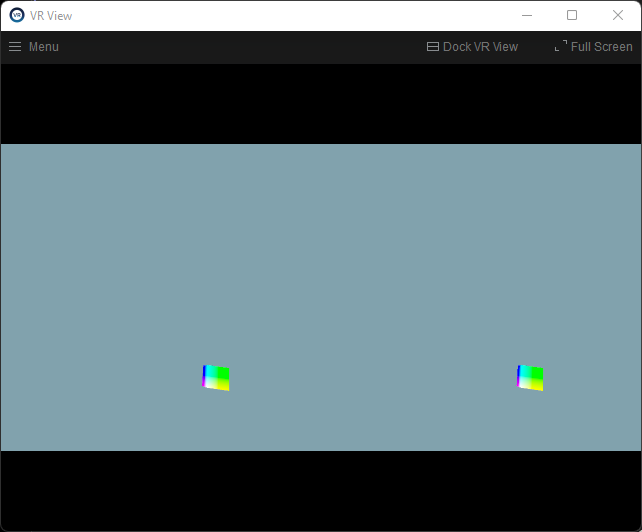
\includegraphics[width=.9\linewidth]{resources/demo_ovvr_1.png}
    \caption{Applicazione demo con OvVR 1}
  \end{minipage}
  \begin{minipage}{.45\textwidth}
    \centering
    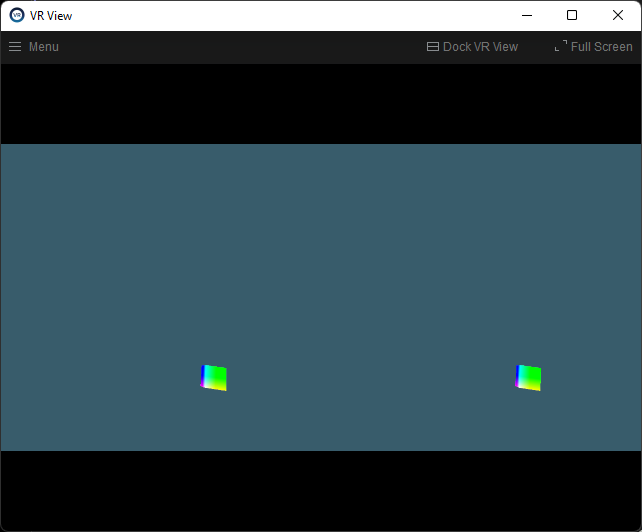
\includegraphics[width=.9\linewidth]{resources/demo_xrbridge_1.png}
    \caption{Applicazione demo con XrBridge 1}
  \end{minipage}
\end{figure}

\begin{figure}[H]
  \begin{minipage}{.45\textwidth}
    \centering
    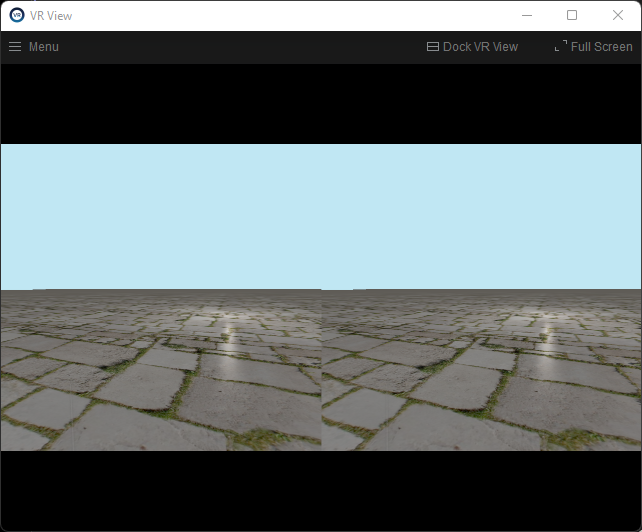
\includegraphics[width=.9\linewidth]{resources/demo_ovvr_2.png}
    \caption{Applicazione demo con OvVR 2}
  \end{minipage}
  \begin{minipage}{.45\textwidth}
    \centering
    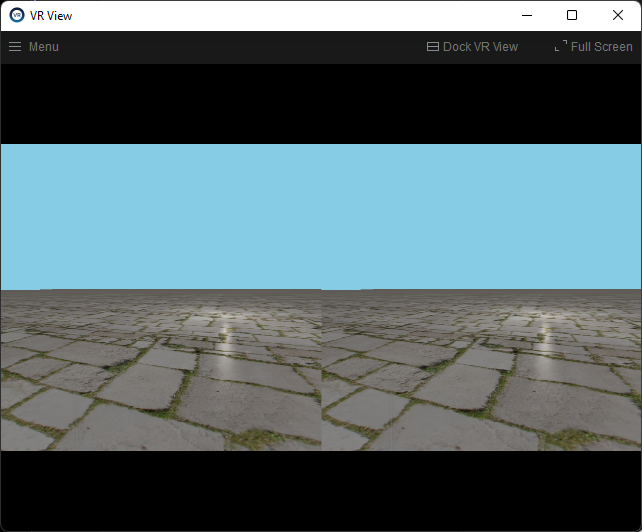
\includegraphics[width=.9\linewidth]{resources/demo_xrbridge_2.png}
    \caption{Applicazione demo con XrBridge 2}
  \end{minipage}
\end{figure}

La differenza dei colori è causato dal formato scelto (RGB vs sRGB).

\chapter{Conclusioni}

Personalmente ho trovato questo progetto molto interessante. Oltre ad avermi permesso di approfondire le mie conoscenze nell'ambiente dello sviluppo, mi ha insegnato soprattutto l'importanza del trovare compromessi fra semplicità d'uso e semplicità di implementazione necessari per sviluppare una API, che verrà utilizzata in un contesto scolastico. Oltre a ciò, con il procedere del mio lavoro, ho potuto provare e sperimentare le difficoltà e le frustrazioni che lavorare su progetti multipiattaforma possono comportare.

Le difficoltà che ho incontrato sono state in buona parte superate e sono state utili per capire gli ostacoli con cui ci si viene a confrontare nella realizzazione di un reale progetto.

Nel mio lavoro ho tentato di fare in modo che XrBridge possa essere facilmente esteso e modificato dal docente e/o dagli studenti per accomodare scenari o cambiamenti futuri.

La realtà virtuale è un campo in continua evoluzione, come pure OpenXR, SteamVR e Linux. Questo significa che alcuni dei problemi riscontrati (per esempio: formati d'immagine supportati) potrebbero venire risolti in un aggiornamento nel vicino futuro.

In conclusione, posso dire di essere soddisfatto con il lavoro svolto e il risultato ottenuto, nonostante le piccole imperfezioni dovute alle differenti piattaforme e formati supportati.

\section{Sviluppi futuri}

XrBridge è stato progettato in modo da permettere l'aggiunta di nuove funzionalità in futuro.

Uno dei potenziali sviluppi futuri è l'implementazione della gestione dell'input. OpenXR permette di gestire l'input generato da vari dispositivi VR e gamepad di vario genere grazie al suo approccio generico. Questo era un requisito opzionale \textit{nice to have} di questo progetto ma, a causa dei problemi menzionati in precedenza, non è stato possibile implementarlo.

Un'altra idea sarebbe quella di adattare XrBridge in modo che sia in grado si supportare più tipi di applicazioni, come ad esempio la realtà aumentata. Questo renderebbe XrBridge più potente e più flessibile e potrebbe essere utilizzato per più applicazioni.

Ci sono inoltre piccoli dettagli che non sono stati implementati poichè non necessari al corretto funzionamento di XrBridge. Questo include la gestioni di alcuni tipi di eventi generati da OpenXR, come ad esempio \texttt{XrEventDataReferenceSpaceChangePending}, il quale indica una modifica dello spazio di riferimento (per esempio causato dalla calibrazione da parte dell'utente), oppure i vari eventi che indicano che la runtime si sta disconnettendo solo temporaneamente e che l'applicazione potrà riconnettersi nuovamente. Non ho mai osservato questi eventi durante lo sviluppo e perciò gli ho considerati di bassa importanza.

Infine, alcuni dei problemi riscontrati, come ad esempio la differenza dei formati supportati fra Windows e Linux, sono problemi che potrebbero venire risolti dagli sviluppatori di SteamVR in un aggiornamento in futuro. È perfettamente possibile che, prima che il corso di realtà virtuale inizi, più formati saranno supportati.

\nocite{*}
\bibliographystyle{unsrt}
\bibliography{document}

\end{document}
